\documentclass[12pt]{article}
\title{Edzőterem működését támogató szoftver PureScript és Vue.js alapokon}
\author{Mezei Botond, Szabó Benedek}
\date{2023}
\renewcommand{\contentsname}{Tartalomjegyzék}
\usepackage[utf8]{inputenc}
\usepackage{graphicx}
\graphicspath{ {./images/} }
\usepackage{wrapfig}
\renewcommand{\figurename}{Ábra}
\usepackage{amsmath}
\usepackage{subcaption}
\usepackage{amssymb}
\usepackage[export]{adjustbox}
\usepackage[magyar]{babel}
\usepackage[breaklinks]{hyperref}
\usepackage{microtype}
\usepackage[T1]{fontenc}
\usepackage{lmodern}
\usepackage{multirow}
\usepackage[table]{xcolor}
%\usepackage{natbib}

\setlength{\arrayrulewidth}{0.5mm}
\setlength{\tabcolsep}{7pt}
\renewcommand{\arraystretch}{2.5}

\textwidth=14cm \textheight=20cm
%\hoffset=-1cm
%\voffset=-1cm

\newtheorem{theorem}{Theorem}[section]
\newtheorem{acknowledgement}[theorem]{Acknowledgement}
\newtheorem{algorithm}[theorem]{Algorithm}
\newtheorem{axiom}[theorem]{Axiom}
\newtheorem{case}[theorem]{Case}
\newtheorem{claim}[theorem]{Claim}
\newtheorem{conclusion}[theorem]{Conclusion}
\newtheorem{condition}[theorem]{Condition}
\newtheorem{conjecture}[theorem]{Conjecture}
\newtheorem{corollary}[theorem]{Corollary}
\newtheorem{criterion}[theorem]{Criterion}
\newtheorem{definíció}[theorem]{Definíció}
\newtheorem{discussion}[theorem]{Discussion}
\newtheorem{example}[theorem]{Example}
\newtheorem{exercise}[theorem]{Exercise}
\newtheorem{explanation}[theorem]{Explanation}
\newtheorem{illustration}[theorem]{Illustration}
\newtheorem{lemma}[theorem]{Lemma}
\newtheorem{notation}[theorem]{Notation}
\newtheorem{problem}[theorem]{Problem}
\newtheorem{proposition}[theorem]{Proposition}
\newtheorem{remark}[theorem]{Remark}
\newtheorem{solution}[theorem]{Solution}
\newtheorem{summary}[theorem]{Summary}

\makeatletter
%\renewcommand*{\@biblabel}[1]{–}
\makeatother

\begin{document}
\begin{titlepage}

	\begin{center}
	\mbox{}\\
	\vspace{35mm}
	\huge
	\textsc{Diplomamunka}
	\end{center}

	
	\vspace{55mm}
	\Large
	\hspace*{\fill} 
	\textbf{Mezei Botond, Szabó Benedek}
	
	\begin{center}
	\vspace{55mm}
	Debrecen\\	
	2023
	
	\end{center}
\end{titlepage}
\begin{titlepage}

	\vspace*{-2cm}
	\hspace*{-1.5cm}

	\begin{center}
	\large
	Debreceni Egyetem
	
	Informatikai Kar	

	Számítógéptudományi Tanszék
	
	\vspace{17mm}
	\huge
	\LARGE
    \textbf{Edzőterem működését támogató szoftver PureScript és Vue.js alapokon}
	
	\vspace{15mm}
	\large
	\textsc{Diplomamunka}
	
	\normalsize
	\vspace{20mm}
	\textsc{Készítette:}
	
	\vspace{5mm}
	\Large
	\textbf{Mezei Botond és Szabó Benedek}
	
	\normalsize
	programtervező informatika szakos hallgatók
	
	\vspace{18mm}
	\textsc{Témavezető:}\\
	\vspace{5mm}
	\large
	Dr. Battyányi Péter \\
	\normalsize
	adjunktus\\
	
	\vspace{32mm}
	Debrecen\\	
	2023
	
	\end{center}
\end{titlepage}
\newpage
\tableofcontents
\newpage
\section*{Bevezetés}
\addcontentsline{toc}{section}{Bevezetés}

A funkcionális programozás egy kevésbé elterjedt programozási paradigma. Noha számos népszerű nyelv használ funkcionális elemeket \cite{Java} \cite{py} \cite{cpp},  a teljesen funkcionális fejlesztés nem annyira népszerű. Megismerése az oktatásban sem igazán hangsúlyos. Ennek ellenére számos előnnyel rendelkezik, melyeket a későbbi fejezetekben fogunk részletezni. Másfajta gondolkosámódot igényel, mint az imperatív megközelítés: a "hogyan?" helyett a "mit csináljon a program?" kérdésre adja meg a választ.

A dolgozatban tárgyalt szoftver backend komponensének elkészítésére a PureScript nyelvet választottuk. Ez egy tisztán funkcionális és erősen típusos programozási nyelv, mely Javascript-re fordul. Azért választottuk ezt a nyelvet, mert tisztán funkcionális, a közelmúltban megjelent nyelv, mely a többi funkcionális nyelvhez (Haskell, Elm) képest modernebb, erőteljesebb, könnyebben használható és teljesebb \cite{CS}.

Munkánk elsődleges célja egy edzőterem működését támogató szoftver elkészítése PureScript backend és Vue.js frontend használatával. Ezen felül szeretnénk megvizsgálni és bemutatni a funkcionális nyelvek használatának előnyeit és lehetőségeit leginkább webalkalmazások fejlesztése során. A szoftver elkészültét követően implementálásra kerül ugyanez a backend Java nyelven a Spring keretrendszer használatával. Célunk a két verzió sebességének és fejlesztési tapasztalatainak összehasonlítása. A sebesség összehasonlítására többféle operációs rendszerrel és különböző specifikációkkal rendelkező számítógépeken ugyanazokat a kéréseket 10, 50 és 100-as kötegekben küldjük el a két különböző szervernek, majd elemezzük az így kapott eredményeket.

A huszonegyedik században egy korszerű edzőteremnek szüksége van egy szoftverre, amely a mindennapi üzletmenetet támogatja. Választásunk azért erre a területre esett, mert egyrészt mindketten szeretünk edzeni járni, másrészt pedig a szoftver összetettsége már alkalmas lehet a PureScript nyelv megismerésére, lehetőségeinek és előnyeinek bemutatására, illetve egy elterjedtebb technológiával (Java, Spring) készült változatával való összehasonlításra.

Az alkalmazás felhasználói az edzőterem recepciós kollégái. A rendszerben lehetőség van rögzíteni:
\begin{itemize}
\item vendégeket
\item bérlettípusokat (jegytípusokat)
\item a felhasználók jegyeit, bérleteit
\item öltözőszekrényeket
\end{itemize}

A\textit{Vendégek} oldalon listázhatjuk a regisztrált vendégeket, újat regisztrálhatunk, a meglévők adatait módosíthatjuk, vendéget törölhetünk. A vendégek számára bérleteket vagy jegyeket lehet vásárolni. A továbbiakban bérletnek nevezzük azt a tagásgot, ami egy időtartamra engedélyezi a terem használatát, jegynek pedig ami alkalmakhoz kötött. A jegyeknek is van egy elévülési ideje. Minden belépőnek három ára van: teljes, diák és klub ár. A felhasználóknak klubtagság vásárlására van lehetőségük, amely különböző előnyökkel jár, például kedvezőbb bérletárak.

A vezérlőpulton lehetőség van a vendégek beléptetésére: a regisztrált vendégek listájából ki kell választani az illetőt. A listában csak az aktív bérlettel vagy érvényes jeggyel rendelkezők jelennek meg. A illetőhöz hozzárendelődik a neme szerint egy szabad öltözőszekrény. Jeggyel rendelkező vendégek számára a jegyen található fennmaradó alkalmak száma eggyel csökken. Az öltözőszekrények megtekintésére egy külön lap szolgál. Itt nemek szerint meg lehet tekinteni minden szekrény állapotát, illetve az előzménytörténetét, vagyis mikor és ki használta. A foglalt szekrények piros színnel jelennek meg.

A vezérlőpulton  a beléptetett vendégek kijelentkeztetésére is van lehetőség. Ezt úgy tehetjük meg, hogy a feljövő listából kiválasztjuk az illetőt. Ilyenkor felszabadul a szekrénye. 

Minden oldal tetején egy navigációs sáv található, mellyel a megfelelő lapra ugorhatunk.

A közös munka során az egyik legnépszerűbb verziókezelő rendszert, a git-et használtuk a Github szolgáltatóval. Az extrém programozás módszerei közül többet is alkalmaztunk, például a páros programozást, mely hatékonynak bizonyult. Lényege, hogy az egyik fejlesztő írja a kódot, a másik pedig segíti közben.

\newpage
\section{Szakirodalmi áttekintés}

\subsection{Funkcionális programozás}
A funkcionális programozás egy programozási paradigma. Több programozási nyelv is tartozik ide, melyeket bizonyos tulajdonságok, módszereik, lehetőségeik, gondolkodási logikájuk köti össze. Az egyik korai funkcionális nyelv a Lisp, melyet John McCarthy alkotott meg az 1950-es évek végén \cite{JM}. Ismertebb funkcionális nyelvek például Haskell, Elm, Erlang, Scala vagy a PureScript. 
A funkcionális programozás során a fejlesztő azt specifikálja a programban, hogy mit kell kiszámítani, és nem azt, hogy hogyan, milyen lépésekben \cite{VD}. A program függvények hívásából és ezek kiértékeléséből áll, nincs értékadás, csak érték kiszámítás \cite{VD}. A függvényt leginkább úgy értjük, hogy egy leképezés egy adott halmazról egy másik halmazra\cite{sy}. A listák (vagy halmazok) kezelésének ezért kiemelt szerep jut a funkcionális nyelvekben. A program tartalmazhat a nyelvben előre definiált, és a programozó által definiált függvényeket. A függvények névvel és opcionálisan argumentumokkal rendelkeznek. Az előállított érték(ek) megegyező paraméterekkel mindig ugyanaz. A rekurzió egy nagyon gyakori koncepció funkcionális nyelvekben.

Egy másik nagy paradigma az imperatív programozás. Az imperatív nyelvek lényege, hogy a programozó a lépéseket definiálja a kódban, melyet a számítógépnek el kell végeznie (utasítások). A legismertebb imperatív nyelv a C.

A logikai programozási paradigma lényege, hogy a programozó állításokat, szabályokat rögzít, melyek használatával a gép automatikusan kikövetkezteti, hogy egy kérdéses állítás igaz, vagy sem. Ilyen nyelv például a Prolog.

Manapság az egyik legelterjedtebb paradigma az objektumorientált programozás. Ez egy gondolkodásmód, tervezési módszer is egyben. A valós világot osztályok formájára képezi le, melynek egyedeit objektumok személyesítenek meg. Legfőbb elvei az egységbezárás (encapsulation: az adatmodell és az eljárásmodell szétválaszthatatlansága), öröklődés (újrafelhasználhatóság kiterjesztése), hozzáférés-szabályozás és többalakúság (polimorphism: lehetővé teszi, hogy ugyanarra az üzenetre különböző objektumok a saját módjukon válaszoljanak) \cite{VD}.

A ma leginkább használatos nyelvekre általánosságban igaz az, hogy nem csupán egyetlen paradigmát követnek tisztán, hanem többet vegyítenek. Ennek az az oka, hogy minden paradigmának megvan a maga előnye (és persze hátránya is), és ezeket az előnyöket érdemes kihasználni. Például a Java (2023. áprilisában a harmadik legtöbbet használt nyelv \cite{TIO}) alapjaiban imperatív, objektumorientált, de a nyolcas verziótól kezdve \cite{Java} megjelennek benne funkcionális elemek, például a lambda kifejezések. A nyelv hivatalos oldala \cite{Java} "erőteljes kiterjesztés"-nek nevezi ezt a lépést.
A Java mellett több elterjedt, nem tisztán funkcionális nyelv, mint például a Python vagy a C++ is épít be funkcionális elemeket \cite{py} \cite{cpp}.

\subsubsection{A funkcionális programozás előnyei}
A funkcionális programozás, mint paradigma, számos előnnyel rendelkezik. Az imperatív gondolkodás kötöttségét egy másfajta megközelítéssel oldja fel. A lényeg, hogy \textit{mit} csináljon a program, és nem az, hogy \textit{hogyan}. Ez az ötlet a programozótól is  másfajta megközelítést, gondolkodásmódot kíván, és máshogy strukturált kódot is fog eredményezni. 

Ránézésre jobban érthető, átláthatóbb, esztétikusabb kód. A szoftver "viselkedése" jobban olvasható \cite{CS}. Ez az előny egyszerűen a funkcionális szintaktikából és gondolkodásmódból adódik. A következő Java kódrészletek Boris Radojicic 2022-es cikkéből \cite{sy} származnak. Az elsőn az iteratív megközelítés látható:

\begin{verbatim}
public List<String> getAddresses(List<Person> persons) {
    List<String> addresses = new ArrayList<>();
    for (int i = 0; i < persons.size(); i++) {
        Person person = persons.get(i);
        if (person.hasValidData()) {
            String address = person.getAddress();
            addresses.add(address.trim());
        }
    }
    return addresses;
}
\end{verbatim}
A következő kódrészlet pedig a funkcionális megközelítést alkalmazza:
\begin{verbatim}
public List<String> getAddresses(List<Person> persons) {
    return persons.stream()
            .filter(person -> person.hasValidData())
            .map(person -> person.getAddress())
            .map(address -> address.trim())
            .collect(Collectors.toList());
}
\end{verbatim}
Míg a két kód ugyanazt a viselkedést eredményezi, a kettőre ránézve elmondható, hogy a második olvashatóbb és tömörebb.

Nagy fokú újrafelhasználhatóság. Mivel egy funkcionális program gyakorlatilag függvények deklarálásából és függvényhívásokból áll, ezeket a függvényeket nagy mértékben újra lehet hasznosítani, elkerülve a feleslegesen duplikált kódrészleteket. A felesleges kód rontja az átláthatóságot és több erőforrást is igényel.

Könnyebb tesztelhetőség. Mivel a funkcionális programban nincsenek állapotok és mellékhatások, így könnyebb lefedni az összes esetet. Illetve ebből kifolyóan, a függvénynek bizonyos bemenő paraméterekre mindig ugyanazt az egyértelmű kimenetet kell előállítania.

A rekurzió hatékony használata. A rekurzió a funkcionális nyelvek gyakori eleme. Átláthatóvá és egyértelművé teszi a kódot teszi a kódot bizonyos problémák esetében, ahol a rekurzív definiálás a természetesebb megoldás. A rekurziónak egy speciális esete a farokrekurzió. Ez azt jelenti, hogy a rekurzív hívás a legutolsó művelet, amit a függvény végrehajt. Nagy előnye, hogy idő és erőforrás takarékos a nem farokrekurzív függvényekkel szemben, ugyanis a fordító kevesebb információt kell, hogy tároljon ilyen módon a veremben.

\subsubsection{A funkcionális programozás nehézségei}

Az előnyök között első helyen állt az átláthatóság és érthetőség. Ehhez viszont hozzátartozik az, hogy a fejlesztő előtte megismerje és elsajátítsa a funkcionális programozás gondolkodásmódját, ami néha bizony nem egyszerű és nem a legtermészetesebb megoldásnak tűnhet.

Memóriahasználat és teljesítmény. Mivel a funkcionális nyelvek nem használnak érték-átadást, sokszor egy változó értékének megváltozása helyett létrejön egy újabb, ami így több erőforrást igényel \cite{JN}. A legtöbb funkcionális nyelv ennek ellenére számos módon ígyekszik ezt kompenzálni: farokrekurzió, lusta kiértékelés, "smart linking". A több paradigmát támogató vagy OOP nyelvek nem feltétlen implementálják ezeket az optimalizációkat \cite{JN}.

Mivel a funkcionális nyelvek használata kevésbé elterjedt, kevesebb eszköz, keretrendszer áll rendelkezésre és kevesebb a felhasználók, szakértők száma. Ennek következtében a fejlesztést nehezíti néha a dokumentáció hiányossága vagy teljes hiánya, illetve az interneten fellelhető minta kódok hiánya és elavultsága.

\subsection{PureScript}

A nyelvet Phil Freeman tervezte 2013-ban, ugyanis nem volt megelégedve a Haskell-t Javascript-re fordító próbálkozásokkal (például Fay, Haste, vagy GHCJS) \cite{pd}. A nyelv teljes forráskódja és dokumentációja megtalálható a GitHubon \cite{pgit}. Hasznos dokumentációs forrás továbbá a Pursuit \cite{purs}, illetve a nyelv alkotója által publikált PureScript by Example könyv \cite{PE}.

A PureScript egy erősen típusos, tisztán funkcionális nyelv. Javascript kódra fordul. Ennek előnye, hogy a kód írására egy szép, könnyen áttekinthető és egyértelmű nyelvet haszálunk, amiből egy hatékony Javascript kód generálódik. Amit Javascriptben meg lehet írni, azt nagyjából PureScriptben is \cite{CS}. A böngészőben és  a szerveren egyaránt futtatható.

A nyelv alapja a Haskell, nagyban hasonlít rá. Maga a szintkaxis annyira hasonló, hogy néhány fejlesztői eszköz a kód megjelenítéséhez a Haskell kiemelését használja. A nyelv fordítója is Haskell nyelven íródott \cite{CS}. Charles Scalfani \cite{CS} szerint erősebb, de egyben könnyebben is használható, mint a Haskell.

A nyelv komoly előnye, hogy frontend és backend fejlesztésre egyaránt alkalmas lehet \cite{CS}.

A PureScriptnek saját csomagkezelő - fordító szoftvere van, a Spago \cite{spago}. Forráskódja szintén elérhető a GitHubon. Munkánk során mi is ezt használtuk, véleményünk szerint nagyon egyszerűen használható, és probléma sem merült fel vele kapcsolatban.

A PureScript rendelkezik egy parancsoros végrehajtási móddal,  ezt PSCI-nek vagy REPL-nek nevezik.  Soronként történik a kód begépelése és végrehajtása. Több sort is megadhatunk egyszerre a \textit{:paste} paranccsal (kilépés: ctrl + D).  A nyelvvel való ismerkedés és a tesztelés során hasznos lehet,  ugyanis lépésről lépésre tudjuk irányítani a kódot,  például típusok lekérdezéséhez. 

A következő kódcsipet a  \textit{Hello,  world!} program PureScript változata:

\begin{verbatim}
module Main where

import Prelude

import Effect (Effect)
import Effect.Console (log)

main :: Effect Unit
main = log "Hello World!"
\end{verbatim}

Előre definiált könyvtárakból lehetőség van függvényeket importálni,  ezt a fájl elején tehetjük meg.  Elég explicit módon kell megadni a konkrét behívandó függvényeket és komponenseket.  Ezután (mint tiszta funkcionális nyelvhez illik) függvények deklarációja és definíciója következik.  A következő kódcsipet egy függvényt ábrázol:

\begin{verbatim}
add :: Int -> Int -> Int
add a b = a + b
\end{verbatim}

Az első sor nem kötelező,  de az átláthatóság érdekében érdemes megadni.  Azt lehet belőle leolvasni,  hogy az add egy olyan függvény,  amely két Int típusú input paraméterrel rendelkezik,  és kimeneti értékként egy Int-et állít elő. A függvény a következőt csinálja: \cite{CS}:
\begin{itemize}
\item kap egy vagy több bemeneti értéket
\item elvégez bizonyos számításokat
\item visszaad egy értéket
\end{itemize}
Egy tiszta függvény mellékhatás mente, és mindig ugyanazt a kimenetet állítja elő\cite{CS}.  A tiszta funkcionális elvek szerint egy függvénynek csak egy kimeneti értéket adhat vissza. Ez nehézségnek tűnhet, de az úgy nevezett \textit{Currying} koncepció segíthet: egy több paraméteres függvény egy paraméteres függvények halmazára cserélését jelenti.

A nyelv további jellemzője, hogy minden változó "Immutable", vagyis a létrejöttük után nem módosulhatnak. Ez is egy érdekes tulajdonság az imperatív világban járatosabb fejlesztők számára.  Az imperatív nyelvekben is van lehetőség objektumoknak ilyen tulajdonság beállítására.  PureScriptben a \textit{let} kulcsszó gyakran segítségünkre lehet ilyenkor, például:

\begin{verbatim}
add :: Int -> Int
add x = do
  let y = 20
    x + 20
\end{verbatim}
A fenti függvény visszaadja a bemeneti értéknél hússzal nagyobb integert. PureScriptben a sorok behúzása is lényeges, a Pythonéhoz hasonló elven működik. Ott, ahol a legtöbb nyelv zárójeleket használna, a PureScriptben behúzás található: eggyel bentebbi behúzás egy zárójelezett blokknak felel meg.

Az imperatív nyelvek egyik alap építőelemét, a ciklusokat is el kell felejteni PureScriptben. Más megközelítés helyettük például a rekurzió használata, mely a funkcionális nyelvekben gyakori koncepció. Példaként Charles Scalfani könyvéből \cite{CS} mutatok két Javascript kódcsipetet, melyek ugyanazt a célt szolgálják. 
A ciklusos megközelítés:

\begin{verbatim}
const factorial = n => {
    var result = 1;
    for (var i = 1; i <= n; ++i)
        result = result * i;
    return result;
};
\end{verbatim}

Funkcionális módon:
\begin{verbatim}
const factorial = n => n === 0 ? 1 : n * factorial (n - 1);
\end{verbatim}

A második kódcsipet úgy definiálja a függvényt, hogy azt mondja meg, \textit{mit} számoljon ki, míg az első a \textit{hogyan} kérdésre adja meg a választ. Ugyanez a kód PureScriptben:

\begin{verbatim}
factorial :: Int -> Int
factorial n =
   if n = 1 then 1 else factorial $ n - 1
\end{verbatim}

A fenti két funkcionális függvény farokrekurzív, mivel a rekurzív hívás maga a függvényben az utolsó hívás. A rekurzió egy előnyös fajtája, mivel kevesebb memóriát igényel. Ez annak köszönhető, hogy ily módon a veremben kevesebb információ tárolódik, és a sebesség is szignifikánsan jobb lesz egy nem farokrekurzív függvényhez képest.

A PureScript továbbá statikus nyelv.  Ez azt jelenti, hogy a típusok ellenőrzése fordítás alatt zajlik, és nem futásidő alatt. Előnye, hogy a hibák már fordítás közben kiderülnek,  kevesebb tesztelés szükséges. Hátránya pedig, hogy a típusokra több figyelmet kell fordítani, limitálja a programozói szabadságot \cite{CS}.

A nyelvvel kapcsolatban kissé negatívum élményként tapasztaltuk, hogy az általános dokumentáltság (nem magának PureScript nyelvnek a dokumentációja, inkább a rendelkezésre álló egyéb oktatási anyagok, könyvek, példák, megválaszolt kérdésekre gondolva) hiányos, sokszor nehéz volt emiatt haladni a fejlesztéssel. Ez véleményünk szerint egyrészt a kevésbé népes funkcionális fejlesztői közösségnek köszönhető, másrészt pedig a nyelv fiatal korának.

\newpage
\subsection{Vue.js}

Dolgozatunk frontend része Vue.js-ben készült,  ezért röviden szeretnénk összefoglalni annak alapjait, tuldajonságait és egy rövid példán keresztül a használatának könnyedségét.

\subsubsection{JavaScript keretrendszerek}

A Vue.js egy klines-oldali keretrendszer, mely a JavaScript programozási nyelvre épül. A JavaScript 1996-os indulása óta mára már megkerülhetetlen része a webnek, a weben található oldalak több mint 95\%-án használatban van valamilyen formában \cite{JS_USAGE}. Az évek során a nyelvvel dolgozó fejlesztőknek köszönhetően számos különböző problémára megoldást nyújtó könyvtár született, mely mind a web mai formájának alakulásához járult hozzá.

A keretrendszerek is ilyen könyvtárak. Meghatározzák egy abban írt szoftver felépítését, mely olyan előnyökkel jár mint a kiszámíthatóság, fenntarthatóság illetve a skálázhatóság.
A keretrendszerek megépítésének motivációja a fejlesztési munkamenet egyszerűsítésében keresendő. Nem vértezi fel új képességekkel az eredeti programozási nyelvet (jelen esetünkben a JavaScriptet), hanem átláthatóbbá valamint könnyebben elérhetővé teszi azt. Általuk a fejlesztőknek csak azt kell meghatározniuk, hogy hogyan nézzen ki az általuk elkészíteni kívánt felhasználói felület, a megvalósításról pedig már a keretrendszer gondoskodik.

Az alább felsorolt tulajdonságok szintén a fejlesztési folyamatok megkönnyítéséhez járulnak hozzá:
\begin{itemize}
\item tesztelési és kódellenőrzési eszközök biztosítása,
\item felhasználói felület részekre (komponensekre) osztása,
\item útvonalkezelés megkönnyítése.
\end{itemize}

Az elvitathatatlan előnyökön felül természetesen van más nézőpont is ami felől vizsgálódnia szükséges egy fejlesztőnek, mielőtt egy keretrendszer használatába kezd, az alap JavaScriptet elfeledve. Fontos észben tartani, hogy a keretrendszerek elsajátításához időre van szükség, hogy az általa biztosított eszközöket a lehető leghatékonyabban tudja felhasználni a fejlesztő a céljai elérésére. Elenghetetlen továbbá átgondoli az elkészítendő program célját. Egy olyan alkalmazás, amely semmilyen felhasználói interakcióval nem rendelkezik, nem biztos, hogy igényel egy olyan professzionális fejlesztői eszközt, mint egy keretrendszer, mely komplex struktúrája feleslegesen bonyolítja a fejlesztési folyamatot.

Ahhoz, hogy az elérhető keretrendszerek közül a legmegfelelőbb kerüljön kiválasztásra, érdemes szem előtt tartani néhány egyszerű szempontot. A választott keretrendszer dokumentációjának minősége és elérhetősége. Minél részletesebb, minél több példával rendelkezik, annál könnyebb lesz a fejlesztés során felmerülő problémákra megoldást találni vagy az implementációs kérdésekben döntést hozni. A dokumentációt kiegészítő szempont a fejlesztői közösség aktivitása, amely a speciális esetekben nyújtat segítséget, akár korábban feltett és megválaszolt kérdéseken keresztül.

\subsubsection{A Vue.js rövid története és tulajdonságai}

A Vue.js ötlete Evan You Google alkalmazott fejében született meg \cite{VUE_BOOK}. A munkája során szüksége lett volna egy olyan hatékony eszközre, ami gyorsan képes nagy mennyiségű HTML dokumentumot előállítani adatok és prototípusok felhasználásával. A már létező eszközök nem tudták teljes mértékben kielégíteni az igényeit \cite{VUE_BOOK}. Volt olyan, amelyik csupán struktúrát biztosított, de az adatkezelése nem volt ideális (Backbone), de volt olyan is, amelyik túl szigorú, kötött szabályrendszerével nem csak a fejlesztendő alkalmazás struktúráját, de a kódolási folyamatot is túlságosan nagy mértékben kívánta befolyásolni (Angular). A megfelelő megoldás hiánya arra késztette, hogy saját maga hozza létre az általa keresett keretrendszert. Így jelent meg a keretrendszer 2014-ben, mely azóta egy lelkes fejlesztő kis magánprojektjéből széles fejlesztői körökben elterjedt és folyamatosan fejlődő keretrendszerré nőtte ki magát.

A Vue.js figyelemre méltó eredménye, hogy fel tudta venni a versenyt olyan elterjedt, szintén JavaScriptre vagy TypeScriptre épülő keretrendszerekkel mint az Angular vagy a React. Ebben hatalmas szerepe van az elérhetőségének. Minden olyan böngésző képes a Vue.js-t kezelni, amelyik támogatja az ES2015 (ES6) JavaScript szabványt \cite{VUE_SUPP}, ezzel a felhasználók 96,09\%-ához jut el \cite{ES2015_USAGE}. Megbízhatóságát biztosítja a több mint 1,5 millió felhasználó világszinten, de olyan nagyvállalatok is használják mint a NASA, Apple vagy a Microsoft \cite{VUE_COMPANIES}.

A Vue.js az alábbi tulajdonságokkal rendelkezik:
\begin{itemize}
	\item[]\textbf{Gyors}
	- Különféle teljesítménytesztek igazolják, hogy gyorsabb keretrendszer mint a rivális Angular vagy React \cite{FRAMEWORK_PERF}.
	\item[]\textbf{Könnyed}
	- Egy Vue.js-ben fejlesztett alkalmazás az úgynevezett \textit{tree-shaking}nek köszönhetően nem tartalmaz olyan beépített könyvtárakat, amiket a fejlesztés során nem használnak, ezzel csökkentve az alkalmazás végős méretét \cite{VUE_LW}.
	\item[]\textbf{Skálázható}
	- A keretrendszer eszköztára lehetővé teszi nagyobb alkalmazások fejlesztését is, melyet a nagy fokú modularitásának köszönhet \cite{VUE_SCALE}.
	\item[]\textbf{Gyorsan tanulható}
	- A részletes dokumentáció, az aktív közösség és az alapos oktató anyagoknak köszönhetően gyorsan elsajátítható a Vue.js használata, melyet a fejlesztés során is megtapasztalhattunk.
\end{itemize}

Ezeken a tulajdonságokon felül nagy előnye a keretrendszernek, hogy egy komponenshez tartozó forráskódok egyetlen jól struktúrált fájlban megtalálhatók. Ez az úgy nevezett \textit{Single-file Component} tulajdonság. A következőkben a keretrendszer dokumentációja \cite{VUE_DOCS} és saját fejlesztési tapasztalataink alapján ismertetjük annak részletesebb tulajdonságait. Egy fájl tartalma a következőképpen alakulhat:
\begin{itemize}
	\item[]\textbf{Sablon}
	- Először a komponens vázát tartalmazó sablont kell megadnunk, ez minden komponens kötelező eleme. Egy HTML alapú sablon szintaxisban adjuk meg a komponensünk vázát, amelyet az alkalmazás futása során fogunk adatokkal megtölteni. Ezt a sablont a \textit{<template></template>} HTML címkék között tudjuk megadni.
	\item[]\textbf{Szkript}
	- A komponens dinamikusságáért felel, az abban megjelenő adatot szolgáltatja a sablon számára. Itt végezhetünk adatlekérést, kezelhetjük a komponenshez tartozó interkaciók mögötti műveleteket. Megadhatjuk a komponens által felhasznált más komponenseket, változókat, de azt is meg tudjuk pontosan határozni, hogy az adott komponens bizonyos életciklusaiban milyen műveletek hajtódjanak végre. A kódokat a már jól ismert, de opcionális  \textit{<script></script>} HTML címkék között tudjuk elhelyezni. 
	\item[]\textbf{Stílus}
	- A komponensekhez természetesen stílust is rendelhetünk, a Cascading Style Sheet (CSS) stílusleíró nyelv segítségével. Arról is dönthetünk, hogy az itt megírt stílusdefiníciók az egész alkalmazásra legyenek érvényesek, vagy csak az adott komponensre a \textit{scoped} kulcsszó megadásával. Webfejlesztői tapasztalataink szerint ez egy igen erős eszköz. A különféle keretrendszerek nélküli fejlesztés során a stílusok nyomonkövetése egy növekvő alkalmazásban egyre nehézkesebb, nem fenntartható kódot tud eredményezni, mely problémát ezzel az apró megoldással könnyen meg lehet előzni. A stílusdefiníciókat az opcionális \textit{<style></style>} HTML címkék között tudjuk megadni.
\end{itemize}

A \textbf{sablon} és a \textbf{stílus} kapcsolata a HTML és CSS kapcsolatából kézenfekvő, egy alap weblaphoz hasonlóan itt is attribútumokat adhatunk a HTML elemekhez, melyekhez általunk definiált stílus szabályok tartoznak. Az adatot szolgáltató \textbf{Szkript} rész kapcsolata a \textbf{sablon}nal már kicsit bonyolultabb, de egy egyszerű példán keresztül könnyen át lehet látni a működést.

\subsubsection{A Vue.js működés közben}

Mielőtt létrehoznánk első komponensünket, először inicializálnunk kell egy Vue.js-nek megfelelő könyvtárstruktúrát. A fejlett eszközök segítségével ez egy nagyon egyszerű feladat. Először szükségünk lesz a Node.js JavaScript futtató környezet legalább 16.0-s verziójára. Amint ez rendelkezésre áll, a környezethez tartozó \textbf{npm} csomagkezelő segítségével egy parancsban tudjuk telepíteni a függőségeket és inicializálni a példa projektünket:
\begin{verbatim}
npm init vue@latest
\end{verbatim}

Itt meg kell adnunk a készítendő projekt néhány alaptulajdonságát. Majd belépve az újonnan létrehozott projekt könyvtárába már létre is tudunk hozni komponenseket.
Nézzük meg egy alapvető komponens forráskódját tartalmazó fájlt az \textit{PageTitle.vue}-t:
\begin{verbatim}
<template>
    <h1>{{ title }}</h1>
</template>

<script>
export default {
    props: ['title']
}
</script>

<style scoped>
h1 {
    margin-top: 50px;
    margin-bottom: 50px;
    text-align: center;
}
</style>
\end{verbatim}

Ez egy olyan újrafelhasználható cím komponensnek a forráskódja, amelyben a címben megjelenő szöveg paraméterezhetőA fájl elején található a \textbf{sablon}. Ebben található egy \textit{h1} HTML elem. Az elem szövege egy dupla kapcsos zárójelben, egy úgynevezett \textit{mustache} sablonban helyezkedik el. Az ott található \textit{title} kulcsszó egy változó, melynek értéke a \textbf{szkript} részben kerül majd meghatározásra. A dupla kapcsos zárójelben egyébként bármilyen érvényes JavaScript kód elhelyezhető, ami további komplex, de mégis egyszerűen érthető megoldásokat tesz lehetővé.

A \textbf{szkript} részben találhatjuk a komponens számára elérhető változókat függvényeket. Ebben a példakódban egyetlen fajta változót láthatunk. A \textit{props} listában olyan változó neveket sorolunk fel, amelyeknek értékét a komponens más komponensekben való használatakor kell megadni. Például ezt a példa komponenst szeretnénk egy oldal komponensében felhasználni, hogy ott egy címet jelenítsen meg, az általunk választott szöveggel. Ezt a következő féle képpen tudjuk megtenni a \textit{PageComponent.vue} fájl sablon részében:
\begin{verbatim}
<template>
    <PageTitle title="Példa cím"></PageTitle>
</template>
\end{verbatim}

Ekkor a \textit{PageTitle} komponens beágyazódik a \textit{PageComponent} oldal komponensbe, és a hozzá kapcsolt \textbf{title} változó értéke "\textit{Példa cím}", ez a cím fog megjelenni a kirenderelt oldalon. Így egy komponens több oldalon is felhasználható, csupán a \textbf{title} változó értékét kell módosítanunk.

A \textbf{stílus} rész pedig egyértelműen megadja, hogy milyen stílusú legyen a \textit{h1} elemünk. Figyeljük meg a \textit{<style></style>} címkében szereplő \textit{scoped} kulcsszót, mely a már említett módon segít a komponensek stílusainak elkülönítésében.

Az elkészült oldal komponenst importálnunk kell az alkalmazásunk belépési pontjául szolgáló \textbf{App.vue} fájlba, melyet JavaScript segítségével fel kell csatolunk egy HTML fájlban lévő elemre. Ezt követően a következő parancsok segítségével tudjuk elindítani az alkalmazásunkat, mely alapértelmezés szerint egy Vite \cite{https://vitejs.dev/} által lokálisan futtatott szerveren teszi elérhetővé alkalmazásunkat:
\begin{verbatim}
npm install
npm run dev
\end{verbatim}

Ennek további hatalmas előnye, hogy így nem kell minden kód változtatás után újraindítanunk a szervert, hanem az automatikusan képes felismerni és megjeleníteni a változásokat, és a fejlesztőnek már csak az alkalmazása további kialakításával kell foglalkoznia.

\subsection{Spring Boot}

Ahhoz hogy a dolgozatunk PureScript nyelven írt backend részét igazán értékelni tudjuk, szükségünk volt egy másik nyelven írt implementációra, amely jó összehasonlítási alapot nyújthat számunkra. Választásunk azért esett a Spring Bootra, mert ezt egyetemi tanulmányaink során már több ízben is megismerhettük, illetve szakmai tapasztalankon keresztül is találkoztunk ezzel a teljesen más nyelven írt eszközzel. Ebben az alfejezetben ezt szeretnénk bemutatni.

\subsubsection{Java}

A Spring alapja az 1995-ben megjelent, jelenleg az Oracle vállalat kezelésében működő ojektumorientált programozási nyelv és platform, a Java \cite{JAVA_ABOUT}. Az alkotójának, James Goslingnak eredeti célkitűzése az "írd meg egyszer, futtasd bárhol" volt \cite{JAVA_BOOK}, ami a hordozhatóság tulajdonságában meg is valósult. Működése a következő képpen alakul \cite{ORACLE_JAVA}:
\begin{enumerate}
\item A fejlesztő megírja a forráskódot a \textit{.java} kiterjesztésű szöveges fájlba.
\item A \textit{javac} fordító a megírt kódból \textit{.class} kiterjesztésű bájtkódokat tartalmazó fájlokat készít
\item E bájtkódokat fogja a Java Virtual Machine (JVM) a számítógép számára érthető utasításokká formálni, ami így végrehajtja a megírt programot.
\end{enumerate}

A nyelv fontosabb tulajdonságai a következők \cite{JAVA_BOOK}:
\begin{itemize}
	\item[]\textbf{Hordozhatóság}
	- A már említett JVM adja a nyelv hordozhatóságát, mely segítségével bármilyen számítógépen lehetséges Java kód futtatása. Mára a Java támogatása szinte magától értetődő és nem csak a fő operációs rendszerek támogatják, de böngészők, telefonok és IoT eszközök is. Így már szinte szó szerint értelmezhető a fentebbi Gosling idézetben szereplő "bárhol".
	\item[]\textbf{Biztonság}
	- Ez fő szempont volt a nyelv kialakításának kezdeteitől fogva. A Java prograok egy alaposan testreszabható jogosultságokkal rendelkező izolált környezetben futnak, ami lehetővé teszi nem megbízható forrásból származó forráskódok, csomagok használatát, anélkül, hogy az kárt okozna a számítógépünkben.
	\item[]\textbf{Dinamikusság és kiterjeszthetőség}
	- A Java kódok osztályokba szerveződnek, melyeket dinamikusan képes betölteni a fordító, akkor amikor azokra szükség van.
\end{itemize}

A nyelv jelentősége tagadhatatlan. A TIOBE indexen az előkelő harmadik helyen szerepel \cite{TIO}, és bár népszerűsége az utóbbi években valamelyest csökkent, biztosan sokáig népszerű lesz még a már meglévő, ebben a nyelvben írt szoftverek és rendszerek miatt. A népszerűség egyik fontos hozadéka a nyelvvel foglalkozó aktív közösség, mely nagyban hozzájárul a nyelv elsajátításának megkönnyítéséhez.

Amennyire népszerű a programozással megismerkedők körében könnyen tanulhatósága miatt, egy-egy alkalmazás fejlesztése gyakran túlságosan bonyolulttá tud válni. E bonyolultság enyhítésére a Java nyelvhez is készültek keretrendszerek. Egy ilyen keretrendszer a Spring, dolgozatunk második backend implementációjának alapja.

\subsubsection{Spring, a Java keretrendszer}

A Spring egy 2003-ban megjelent keretrendszer Java alkalmazások fejlesztésének támogatásához. Széleskörű eszköztárral rendelkezik, hogy skálázható, nagy teljesítményű alkalamzásokat lehessen általa létre hozni. A keretrendszer legfőbb tulajdonsága a modularitás. Az alap modulon túl a fejlesztő kezében van a döntés, hogy az adott alkalmazásba mely számára szükséges modulokat építi be. A főbb modulok a következő területeket érintik \cite{SPRING_BOOK}:
\begin{itemize}
\item adatelérés és kezelés,
\item web,
\item biztonság,
\item tesztelés.
\end{itemize}

A keretrendszer alapelve a függőség befecskendezés vagy angolul Dependency Injection, melynek lényege, hogy a függőségek futási időben kerülnek átadásra. Ez két alapvető Java koncepció felhasználásával került implementálásra: az interfészek és a JavaBean-ek. Az interfészek és a függőség befecskendezésének kölcsönösen hasznos együttműködésének eredménye a rugalmas de nem túl bonyolult alkalmazások. A függőség befecskendezés előnyei \cite{SPRING_BOOK}:
\begin{itemize}
	\item[]\textbf{Csökkent kódméret}
	- A függőség befecskendezés következtében sokkal kevesebb kódra van szükség ahhoz, hogy alkalmazásunk különböző részeit összeillesszük.
	\item[]\textbf{Alkalmazás konfigurációk egyszerűsödése}
	- A konfigurációk - hasonlóan a Spring alapgondolatához - modulárisan működnek, így ha egy részét le szeretnénk cserélni az alkalmazásunknak, azt nagyon könnyen meg tudjuk tenni.
	\item[]\textbf{Tesztelhetőség fejlődése}
	- Az előbb említett modularitás hozadéka a tesztelésben is tetten érhető. A tesztelési folyamat során a különböző objektumok mock-olása ennek következtében nagyban leegyszerűsödik.
\end{itemize}

\subsubsection{A Spring Boot projekt}

A Spring keretrendszer egy elterjedt modulja a Spring Boot. Erőssége, hogy a korábban említett konfigurációk terhének tetemes részét leveszi a fejlesztők válláról. Az alkalmazásfejlesztésben fontos szerepe van annak is, hogy a Spring boot rendelkezik beépített web szerver támogatással, mint a Tomcat vagy a Jetty, amely lehetővé teszi a Java alkalmazásokból készített JAR csomagok könnyed kihelyezését. Így a fejlesztőnek egy külön álló szerver felállításával sem kell törődnie. Alap csomagokkal is rendelkezik a keretrendszer, amelyek általános felhasználási eseteket fednek le, így egy alap váz létrehozása az alkalmazásunkhoz igazán egyszerű feladat.

Egy Spring Boot alkalmazás felépítése rétegekből áll, mely tartalmazza a következő fontosabb rétegeket:
\begin{itemize}
	\item[]\textbf{Modell}
	- Az alkalmazásban használt entitások modelljeit tartalmazza.
	\item[]\textbf{Perzisztencia}
	- Az entitások és az adatbázis közötti kapcsolatot hozza létre.
	\item[]\textbf{Szolgáltatás}
	- Az entitásokkal kapcsolatos műveleteket adja meg a Perzisztencia réteg felhasználásával.
	\item[]\textbf{Kontroller}
	- Az alkalmazás végpontjaihoz rendeli a Szolgáltatás réteg műveleteit.
\end{itemize}

A Spring Boottal való fejlesztés egyszerűségének ékes példája a Spring által biztosított inicializáló eszköz, a Spring Initializr \cite{SPRING_INIT}. Ebben az eszközben magunk konfigurálhatjuk a készítendő projektünket a projekt menedzsment eszköz, a Spring Boot verzió, a Java verzió vagy az egyéb függőségek kiválasztásával. Ezt követően legenerálódik a projekt a paraméterek alapján, és kezdődhet is a fejlesztés.

E tulajdonságaival rengeteg időt spórol meg a fejlesztők számára, de természetesen ennek ára is. Mivel a lehető legtöbb mindent a fejlesztő helyett kíván megoldani, így a korábban felsorolt előnyöket kevésbé lesz képes kihasználni a fejlesztő, amennyiben egy komplexebb alkalmazást kíván fejleszteni, ezért ilyenkor gyakran kell manuális konfigurációkra támaszkodni az alapértelmezettek helyett.

A hátránya ellenére is hatalmas népszerűségnek örvend, ma is gyakori felhasználási területe a REST API-k fejlesztése, ahogy ez a mi esetünkben is így történt. A saját fejlesztési tapasztalatokon keresztül pedig a fent említett előnyökre és hátrányokra is igazolást fogunk látni.

\newpage
\section{A fejlesztés bemutatása}

A fejlesztés során szem előtt tartottuk azt az elvet,  hogy a két alkalmazás majd nemcsak hogy ugyanazt a funkcionalitást lássa el, de lehetőleg (már amennyire a nyelvi sajátosságok engedik) ugyanúgy is épüljön fel, ugyanúgy viselkedjen.  Mindkét alkalmazás ugyanazt a MySQL adatbázist és ugyanazt a frontendet használja.

Az első lépés az üzleti logika átgondolása, a funkcionális tervezés volt. Mivel a szoftver nem egy valós üzleti igényt elégít ki, hanem inkább kísérleti jellegű (Proof of Concept), így ez a szakasz kisebb hangsúlyt kapott.

Az adatbázis megtervezésével kezdtük. A MySQL adatbáziskezelőt választottuk, mivel nyílt forráskodú, a tervezett funkcionalitást bőven ellátja és könnyen lehet használni. Elkészítettük a sémát, mely az első ábrán látható. Tartalmazza a táblák nevét,  az attribútumokat,  félkövér kiemeléssel az elsődleges kulcsot. A táblák közötti nyilak a külső kulcsokat és kapcsolattípusokat mutatják.

A \textit{Vendégek} tábla tartalmazza egy vendég adatait stb.... ez kell?

\begin{figure}[h!]
\centering
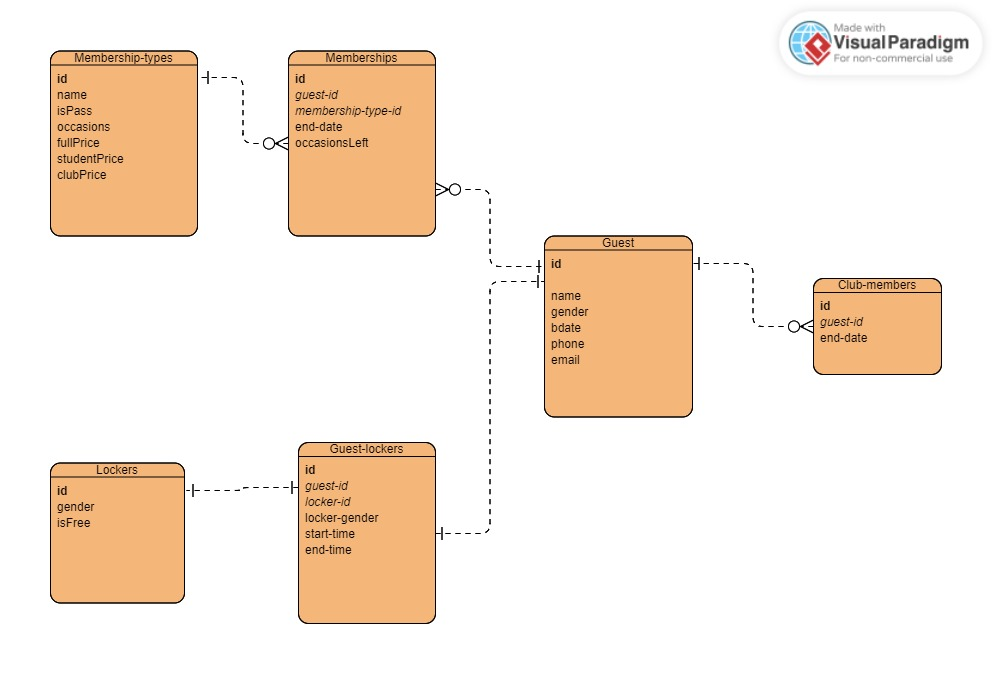
\includegraphics[width=0.8\textwidth]{database}
\caption{A szoftver adatbázis modellje.}
\end{figure}

\begin{figure}[h!]
\centering
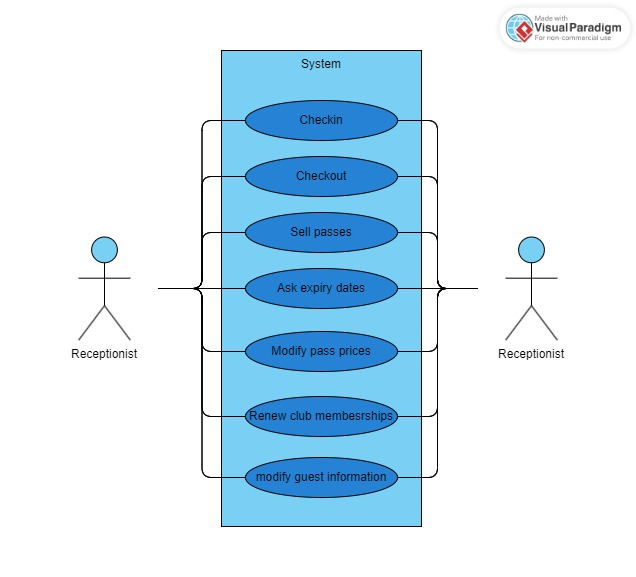
\includegraphics[width=0.6\textwidth]{usecase}
\caption{Használati eset (use case) diagram. }
\end{figure}


A Vue.js-ben implementált frontend ugyanazon a porton (3000, természetesen nem egyszerre) tud kommunikálni akár a PureScript,  akár a Spring Boot REST API-val. Ez HTTP kérések használatával történik: mindkét backend ugyanazokra a kérésekre ugyanazt a választ és ugyanazt a működést eredményezi.  Az első táblázatban néhány kérés látható a vendégekkel kapcsolatban. A szerver erre a kérésre küld egy választ, mely ha szükséges, tartalmazhat a body-ban egy JSON-t.

\begin{table}[h!]
\centering
\begin{tabular}{ |p{1.7cm}|p{4.4cm}|p{6.3cm}| } 
\hline
 \textbf{Metódus} & \textbf{Útvonal} &\textbf{Leírás}\\
\hline
GET & /guest/getAll& Az összes vendég lekérése.\\
\hline
GET & /guest/getById/\{id\}& Egy vendég lekérése az azonosítója alapján.\\
\hline
POST & /guest/insertGuest&  Egy új vendég hozzáadása. \\
\hline
PUT & /guest/updateGuest/\{id\} & Egy vendég kartonjának szerkesztése \\
\hline
DELETE & /guest/deleteGuest/\{id\} & Egy vendég törlése  \\
\hline
... & ... &...  \\
\hline
\end{tabular}
\caption{A kérések listájának részlete.}
\end{table}


Az Uizard\cite{uizard} nevű szoftverrel elkészítettük az oldalak kinézetének terveit, illetve az oldalak közötti navigációt modellező prototípust. Ez nagyon hasznos lehet a korai tesztelés szempontjából, ugyanis egy ilyen prototípus rövid idő alatt elkészíthető, így nagyon hamar egy kattintgatható prototípuson lehet kipróbálni, hogy az üzleti logikának megfelel-e. A harmadik ábrán az így elkészült navigációs térkép és mellette néhány képernyőkép terv látható.
\begin{figure}[h!]
\centering
\begin{subfigure}{0.45\textwidth}
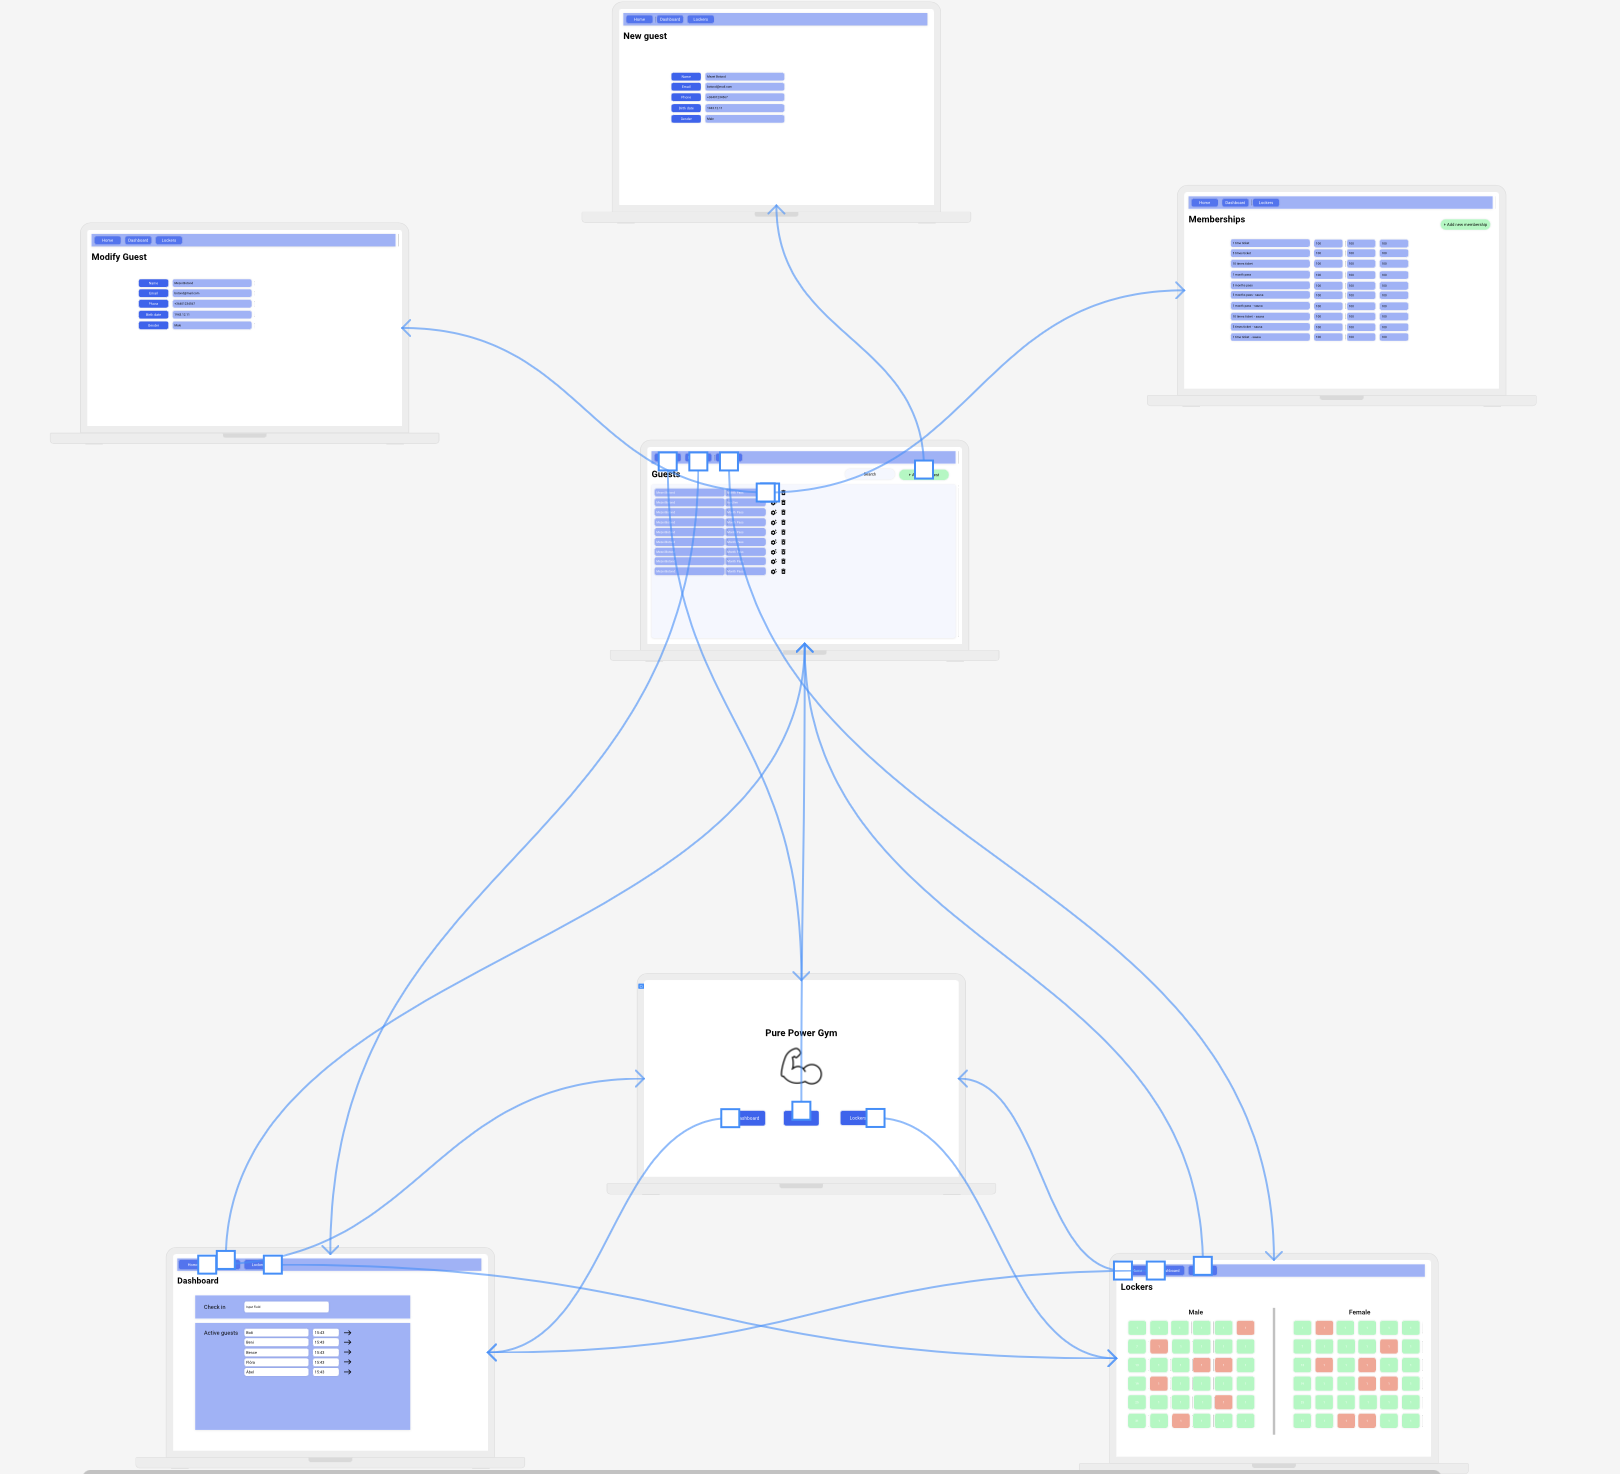
\includegraphics[width=7cm]{navigation} 
\end{subfigure}
\begin{subfigure}{0.4\textwidth}
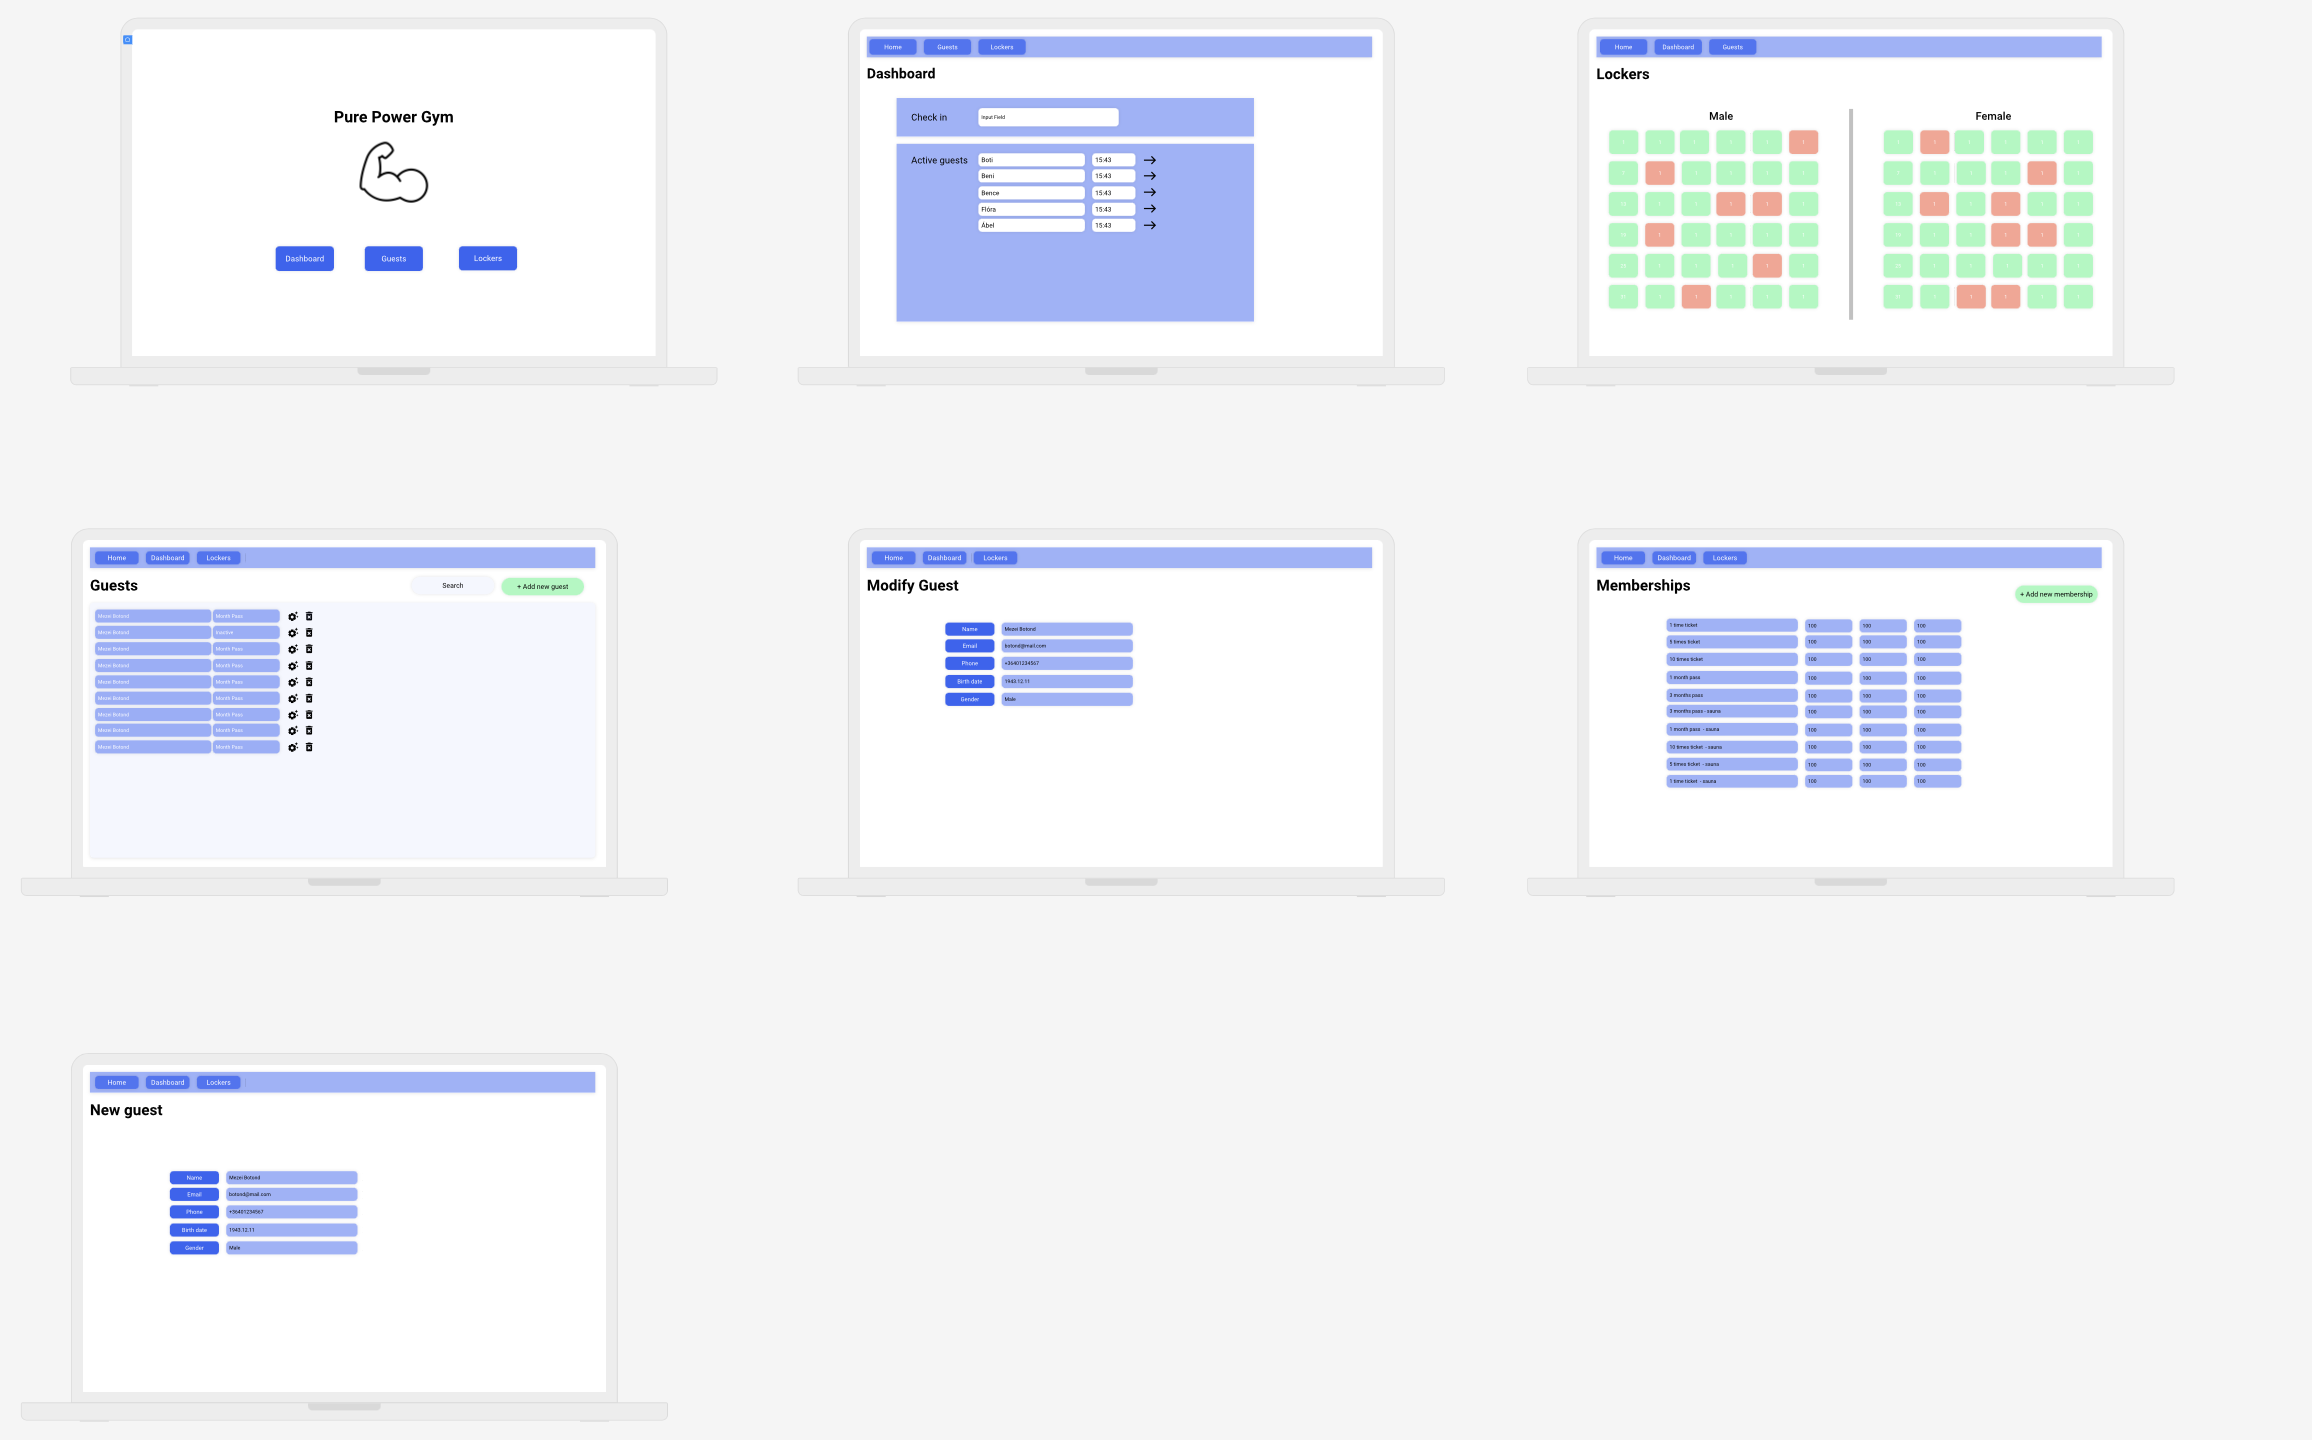
\includegraphics[width=7cm]{pages}
\end{subfigure}
\caption{Az oldalak közötti navigáció és az oldalak tervezése.}
\end{figure}

\newpage
\subsection{PureScript}

Az alkalmazás fejlesztéséhez első lépésként telepítettük a szükséges szoftvereket a npm csomagkezelő segítségével. 
\begin{verbatim}
npm install -g purescript
npm install -g spago
\end{verbatim}

Az első sor maga a PureScript, a második pedig Spago telepítéséhez szükséges. A Spago egyrészt a csomagokat is kezeli, illetve a szoftver életciklusát is menedzseli, például az \textit{install, build, run} parancsok segítségével.  Fejlesztő környezetként a Visual Studio Code-ot választottuk, mely rendelkezik PureScript kiterjesztésekkel és kiemeléssel is.

Ezután jó darabig ismerkedtünk magával a nyelvvel, mivel valamennyi funkcionális tapasztalattal mindketten rendelkeztünk korábban, de nagyrészt imperatív nyelveket használunk.  Ehhez jó segítség volt a PSCI, amit a \textit{spago repl} paranccsal lehet elindítani. Lehetőség van egy alap kód megadására, ami minden indításnál lefut, ide helyeztük a szükséges importokat. Ezután soronként futtattuk a programot, példáuk gyakran lekértük az elemek típusát a \textit{:type} paranccsal.

A következő lépés az üzleti logika átgondolása, a funkcionális tervezés volt. Mivel a szoftver nem egy valós üzleti igényt elégít ki, hanem inkább kísérleti jellegű (Proof of Concept), így hatalmas hangsúlyt nem kapott ez a szakasz. 

A szoftver alapvetően az MVC (model - nézet - vezérlő) architektúrális mintát követi.  A modell megalkotásával kezdtük, ehhez készítettünk egy adatbázismodellt, mely az első ábrán látható. A PureScript kódban ez szolgált a típusok vázaként is. Minden típushoz egy \textit{.purs} fájlt készítettünk, melyben magának a típusnak és a hozzá tartozó függvényeknek a leírása található. A következő módon készítettünk egy ilyen típust:

\begin{verbatim}
newtype Guest = Guest
    { id   :: Int
    , name :: String
    , gender :: String
    , bdate :: String
    , phone :: String
    , email :: String
    }
\end{verbatim}
?readforeign
Egy Guest típusú elemet a következőképp hozhatunk ezután létre repl-ben:
\begin{verbatim}
g = Guest {id:1, name: "Doma" gender:"male", bdate:"2005.04.26", phone:"+36401234567", email:"doma@mail.com"}
\end{verbatim}

\begin{verbatim}
getGuestId :: Guest -> Int
getGuestId (Guest guest) = guest.id
\end{verbatim}

\begin{verbatim}
setGuestId :: Int -> Guest -> Guest
setGuestId s (Guest guest) = Guest {id:s, name:guest.name, gender:guest.gender, bdate:guest.bdate, phone:guest.phone, email:guest.email}

\end{verbatim}

\subsection{Java - Spring Boot backend}

Ebben az alfejezetben az összehasonlítás alapjául szolgáló Java Spring Boot REST API fejlesztését fogjuk bemutatni. Fontos megjegyezni, hogy ha csupán a Spring segítségével szerettük volna elkészíteni a REST API-nkat, akkor valószínüleg nem mindenhol a most implementált megoldásokat alkalmaztuk volna. Mindent olyan módszerrel kívántunk megoldani, ami a legjobban hasonlít a PureScriptben használtakra, mindezt azért, hogy a dolgozatban szereplő összevetésben szereplő különbségek inkább a nyelvbeli különbségekből fakadjanak és ne a megoldások különbségéből. Ez növeli az összehasonlítás értékét, eredményének jelentőségét. Ennek tudatában vegyük végig a fejlesztés lépéseit.

\subsubsection{A tényleges implementáció}

A Java projekt első lépéseként a már említett Spring Initializr eszközt használtuk fel. Ennek három fontos részét kell kiemeljük:
\begin{itemize}
	\item[]\textbf{Projekt menedzsment eszköz: Maven}
	- Mivel mindkettőnk ezt az eszközt használta korábbi Java fejlesztéseink esetén, ezért ezt részesítettük előnyben.
	\item[]\textbf{Java verzió - 8}
	- Azért választottuk ezt a verziót, mert korábban ezzel már fejlesztettünk, illetve a magasabb verziók által kínált nyelvi eszközöket sem kívántunk igénybe venni.
	\item[]\textbf{Függőségek}
	- Szükségünk volt a Spring Boot által biztosított kezdő csomagok közül a \textit{web}-hez kapcsolódóra, az adatbázis eléréshez a \textit{Java Persistence API}-ra (\textit{JPA}), a \textit{MySQL} adatbázishoz kapcsolódáshoz egy \textit{kapcsoló} csomagra és a \textit{Lombok Projekt} csomagjára, melynek a fejlesztési menetre való pozitív hatásáról említést fogunk tenni a későbbiekben.
\end{itemize}

Ezt követően rendelkezésünkre is állt a projekt váza. A következő lépésben kihasználva a Spring konfigurációinak erősségét, elvégezzük a  szükséges konfigurálásokat. Meghatározzuk, hogy a HTTP szerver saját számítógépünk melyik portján legyen elérhető, illetve megadjuk a korábban létrehozott MySQL adatbázisunk elérési adatait és a perzisztálási stratégiát. amely a JPA adatbázisunkhoz való alapvető hozzáállását szabályozza.

Ezután kerültek implementálásra az adatbázisunk tábláiban szereplő entitások modelljei. Meghatároztuk azok attribútumait típusaikkal együtt, mindezeket privát eléréső változók formájában. Az adott entitásokat leképező osztályokhoz szükséges konstruktorok, illetve a változók elérését és beállítását elvégző függvényeinket a már említett Lombok Projekt segítségével, csupán néhány annotáció felhasználásával meg is tudjuk adni. Így az entitások kódja tömör, kompakt marad. Ilyen annotációk a \textbf{@Data} vagy az \textbf{@AllArgsConstructor}. A Spring konfigurálhatósága az entitásoknál is tetten érhető, szintén annotációkon keresztül. Az \textbf{@Entity} annotáció jelzi, hogy az osztály leképezhető az adatbázis egy táblájára, illetve a változók közül az \textbf{@Id} annotáció segítségével adhatjuk meg a leképezett tábla elsődleges kulcsát. Speciális esetben előfordulhat, hogy egy tábla összetett, több mezőből álló elsődleges kulccsal rendelkezik, mely problémát szintén egy egyszerű annotációval, az osztályra helyezett \textbf{@IdClass}-szal tudjuk megoldani, így a változók közül már több kulcsot is ki tudunk jelölni. Nézzük meg a \textbf{Guest} entitást példaként, hogy milyen tömören és egyszerűen lehet lemodellezni az adatunkat:
\begin{verbatim}
@Data
@Entity
@AllArgsConstructor
@NoArgsConstructor
public class Guest {

    @Id
    private Long id;
    private String name;
    private String gender;
    private String bdate;
    private String phone;
    private String email;
}
\end{verbatim}

Az entitásokat követik a hozzájuk tartozó perzisztencia rétegek, ezt minden entitáshoz szükséges megadnunk. Ezek olyan interfészek, mely a \textit{JpaRepository} osztály terjesztik ki, és az entitás struktúrája alapján alapértelmezett SQL lekérdezéseket biztosítanak számunkra Java függvények formájában.  Itt szükséges egy Spring annotáció, a \textbf{@Repository} alkalmazása. Természetesen egyéni lekérdezéseket is hozzá tudunk adni, azonban ennek két alapesete van:
\begin{itemize}
	\item[]\textbf{1. A perzisztencia típusa megegyezik az egyéni lekérdezés eredményének típusával}
	- Ebben az esetben csak a függvényeket kell deklarálnunk és ellátnunk azokat a \textbf{@Query} annotációval, amiben az SQL lekérdezésünket tudjuk elhelyezni. Ezekben természetesen paramétereket is elhelyezhetünk, melyek a későbbiek folyamán töltődnek fel tartalommal.
	\item[]\textbf{2. A perzisztencia típusa nem egyezik meg az egyéni lekérdezés eredményének típusával}
	- Ebben az esetben elegáns megoldásként egy úgynevezett csomagoló osztályt hozhatunk létre, amely a lekérdezési eredmény mezőinek megfelelő változókat tartalmazza, majd ezt követően egy konfigurációs annotáció, az \textbf{@SqlResultSetMapping} hozzáadásával tudathatjuk a Springgel, hogy miként szeretnénk leképezni a kapott eredményt a csomagoló osztály változóira. Ezen apró módosításokat követően viszont ugyanúgy tudjuk megadni az egyéni lekérdezéseinket, mint az előző esetben.
\end{itemize}

A következő réteg a szolgáltatás. Itt adhatjuk meg azokat a függvényeket minden egyes entitáshoz külön osztályban, amelyek a különböző URL-ekre való hívásokkor fognak lefutni. Felhasználjuk bennük a perzisztencia réteg biztosította függvényeket és az egyénileg írt SQL lekérdezéseket is az \textbf{EntityManager} osztályon segítségével. Ehhez a réteghez is kapcsolódik egy Spring annotáció, a \textbf{@Service}. Ebben a rétegben érhetjük tetten a Spring nagy fegyverét, a függőség befecskendezést is. Minden egyes a rétegben használt perzisztencia osztályt definiálnunk kell az \textbf{@Autowired} annotációval együtt. Így a függőségek, nevezetesen a perzisztencia osztályok futási időben lesznek elérhetőek a szolgáltatás osztályokban.

Az utolsó, legfelső réteg pedig a kontroller. Itt már több annotációval találkozhatunk, ezeket vizsgáljuk meg egy példán keresztül:
\begin{verbatim}
@CrossOrigin(origins = "http://localhost:5173")
@RestController
@RequestMapping("/guest")
public class GuestController {

    @Autowired
    GuestService guestService;

    @GetMapping(path = "/getAll")
    List<Guest> getGuests() {
        return guestService.getAllGuest();
    }

    ...
}
\end{verbatim}

Az első annotáció a \textbf{@CrossOrigin}, melyben megadhatjuk, hogy milyen címekről fogadja a kontroller a kéréseket, más címekről érkező kérések elutasításra kerülnek. Itt a mi frontend szerverünk címét adtuk meg, ezzel biztosítva annak a HTTP szerverhez való hozzáférést. A \textbf{@RestController} annotációval tudatjuk a Springgel, hogy az osztály egy kontroller feladatát hivatott ellátni. A \textbf{RequestMapping} annotáció pedig segít nekünk rendszerezni a kontrollerek által adott végpontokat. Itt a vendégekkel kapcsolatos API végpontjaink vannal, ezért az annotációban megadott "\textit{/guest}" biztosítja azt, hogy a felsorolt végpontok ezzel az útvonallal fognak kezdődni a tényleges szerveren. Itt is találkozunk a függőség befecskendezéssel, de itt most a szolgáltatás osztályt szeretnénk befecskendezni, ugyanis az tartalmazza a szükséges függvényeket.

Alatta pedig pegig egy példa végpont látható. Szintén annotáción keresztül tudjuk megadni az elvárt HTTP metódust, illetve az erre a vépontra érvényes útvonalat. Ez a vépont például a szolgáltatás felhasználásával az adatbázisban megtalálható vendégek listáját adja vissza. A korábban említett \textbf{@RestController} annotáció azt is biztosítja számunkra, hogy a függvények eredménye képpen kapott objektumok a HTTP válaszban JSON formátumban jelenjenek meg.

Az összes réteget pedg maga az alkalmazás osztály fogja összekötni, mely osztály rendelkezik a \textbf{@SpringBootApplication} annotációval, és a \textit{main} függvényben csupán egyetlen függvényhívás található:
\begin{verbatim}
SpringApplication.run(PuregymBackendApplication.class, args);
\end{verbatim}

Az egyetlen hiányzó komponense a HTTP szerverünknek egy alkalmazásszerver. A mi megoldásunkban a \textit{Jetty} alkalmazásszervert használtuk fel, és mivel a Spring rengeteg mindent ad alapértelmezetten, így ezt sem kellett külön konfigurálni vagy létrehozni.

Így már minden készen áll arra, hogy elindítsuk a szervert, melyet egy egyszerű \textit{Maven} paranccsal tehetünk meg:
\begin{verbatim}
mvn clean install spring-boot:run
\end{verbatim}

Így az alkalmazásunk néhány másodperc után már elérhető is az általunk konfigurált porton.

\subsection{Vue.js}

A most következő alfejezetben végül pedig a frontend alkalmazásunkként szolgáló Vue.js alkalmazás implementációját mutatjuk be. Mivel mindkét korábban ismertetett backend alkalmazásunk a számítógépünk 3000-es portján futtatható, így a Vue.js alkalmazás mindkét implementációval tökéletesen működik. Fontos megemlítenünk, hogy a dolgozatunknak nem az a célkitűzése, hogy egy tökéletes edzőtermi szoftvert hozzunk létre, hanem megvizsgáljuk a PureScript nyelvű implementációnkat a Spring implementáció tükrében. Így az alkalmazás frontend részének feladata inkább a szemléltetés, mintsem egy létező edzőtermi menedzsment szoftver alternatívája.

\subsubsection{A Vue.js implementáció}

A Vue.js fejlett keretrendszer lévén szintén biztosít számunkra egy egyszerű módot, hogy a fejlesztés zökkenőmentesen kezdődhessen. A projekt vázát a már korábban említett módon kaptuk meg az előző fejezetben említett függőségek telepítése után:
\begin{verbatim}
npm init vue@latest
\end{verbatim}

Alkalmazásunkban a következő főbb oldalakat szeretnénk létrehozni:
\begin{itemize}
	\item[]\textbf{Kezdőlap}
	- Ezzel az oldallal találkozik a felhasználó először, innen lehetősége van továbbnavigálni a többi oldalra.
	\item[]\textbf{Vezérlőpult}
	- Ezen az oldalon lehet nyomon követni az éppen az edzőteremben tartózkodó úgynevezett aktív vendégeket, ki lehet őket jelentkeztetni, illetve itt lehet bejelentkeztetni az aktív bérlettel rendelkező, de nem aktív vendégeket.
	\item[]\textbf{Vendégek}
	- Itt láthatjuk az összes vendéget, aki valaha az edzőteremben járt. Lehet kezelni az adataikat, a Klub tagságukat, a bérleteiket és törölhetjük is őket. Ezen felül új vendég regisztrálására is van lehetőség.
	\item[]\textbf{Öltözőszekrények}
	- Végül itt pedig az öltözőszekrények állapotát tudjuk itt nyomonkövetni. Láthatjuk nemek szerinti bontásban, hogy melyek foglaltak, illetve egy-egy öltözőszekrényre vonatkozóan a használati történetét is megtekinthetjük.
\end{itemize}
\begin{figure}[h!]
	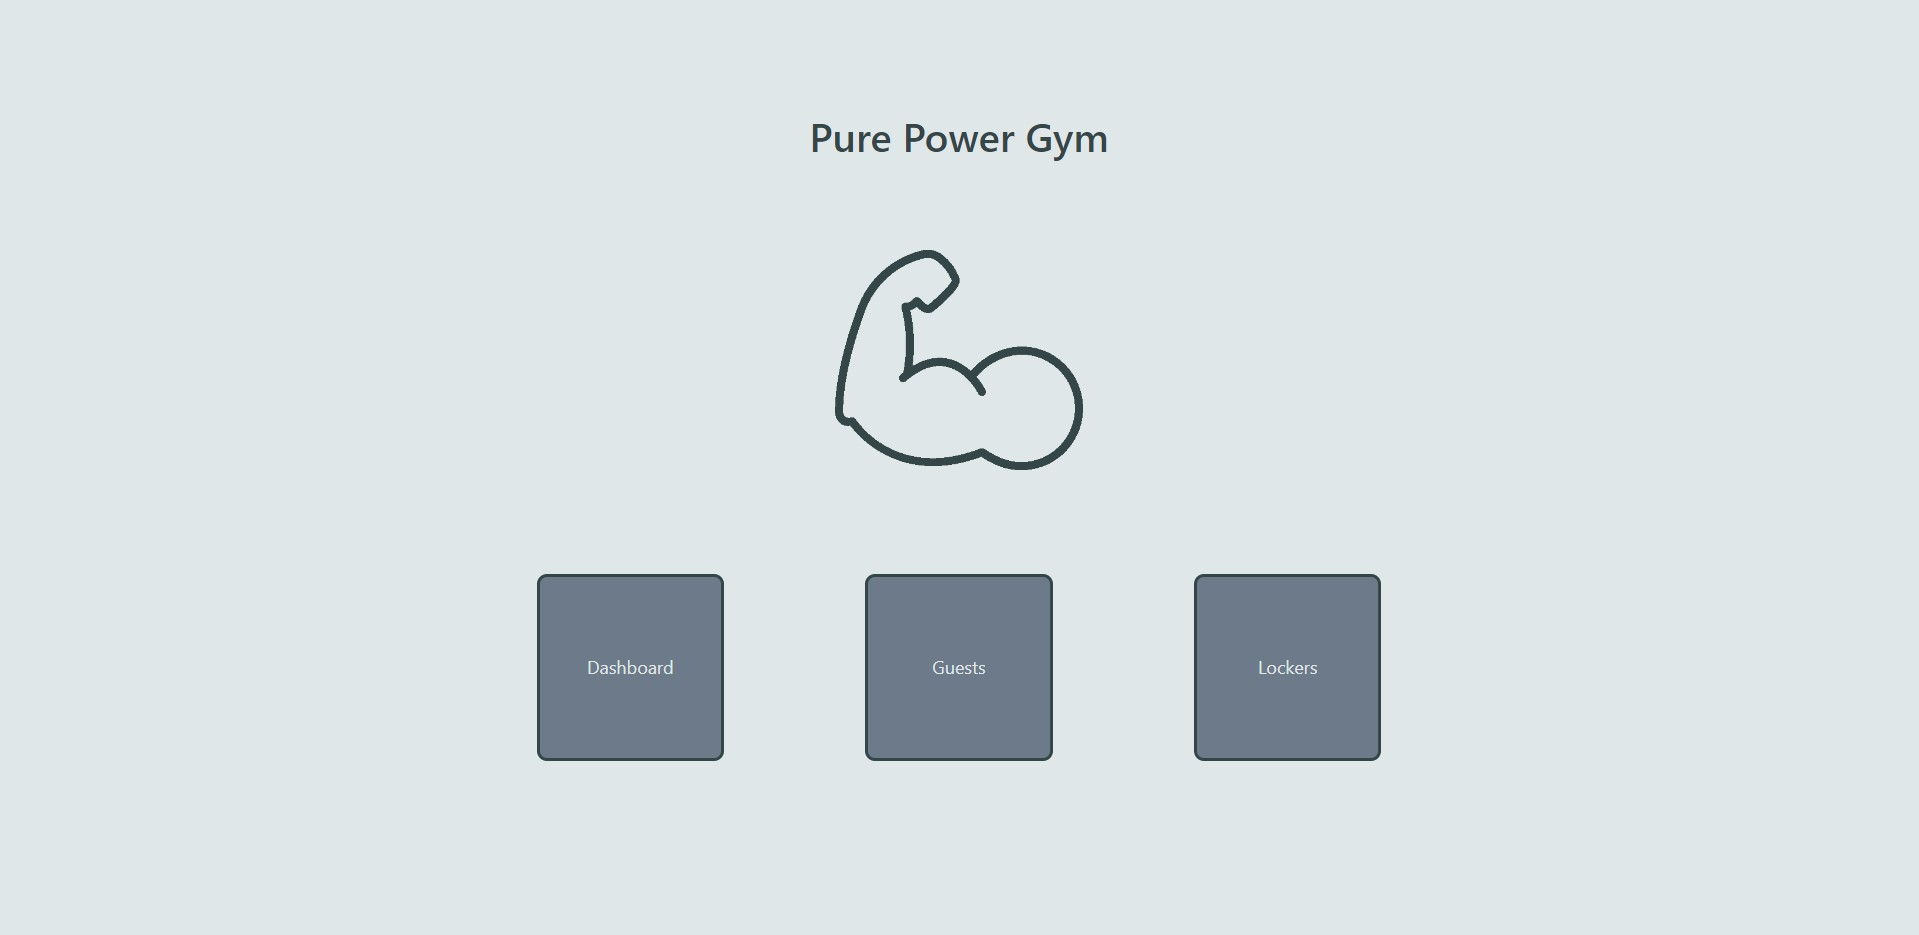
\includegraphics[width=\textwidth]{landing-page}
	\caption{A kezdőlap. }
\end{figure}
\begin{figure}[h!]
	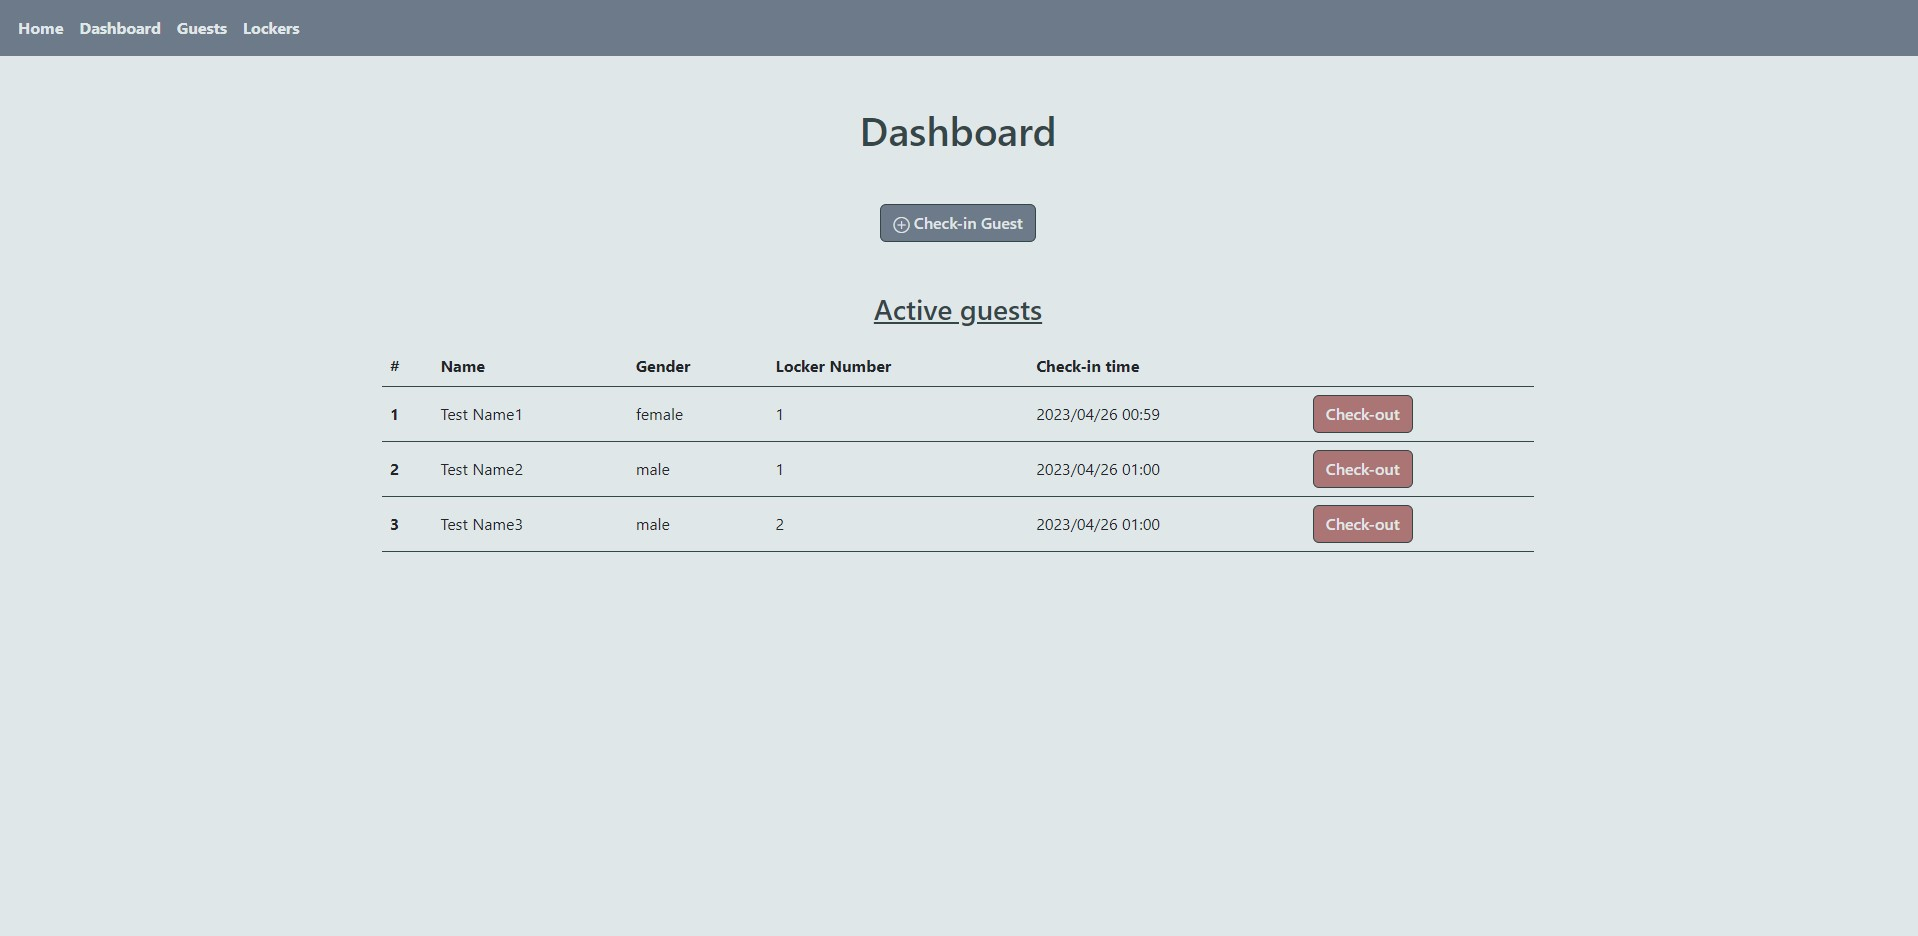
\includegraphics[width=\textwidth]{dashboard-page}
	\caption{A vezérlőpult. }
\end{figure}
\begin{figure}[h!]
	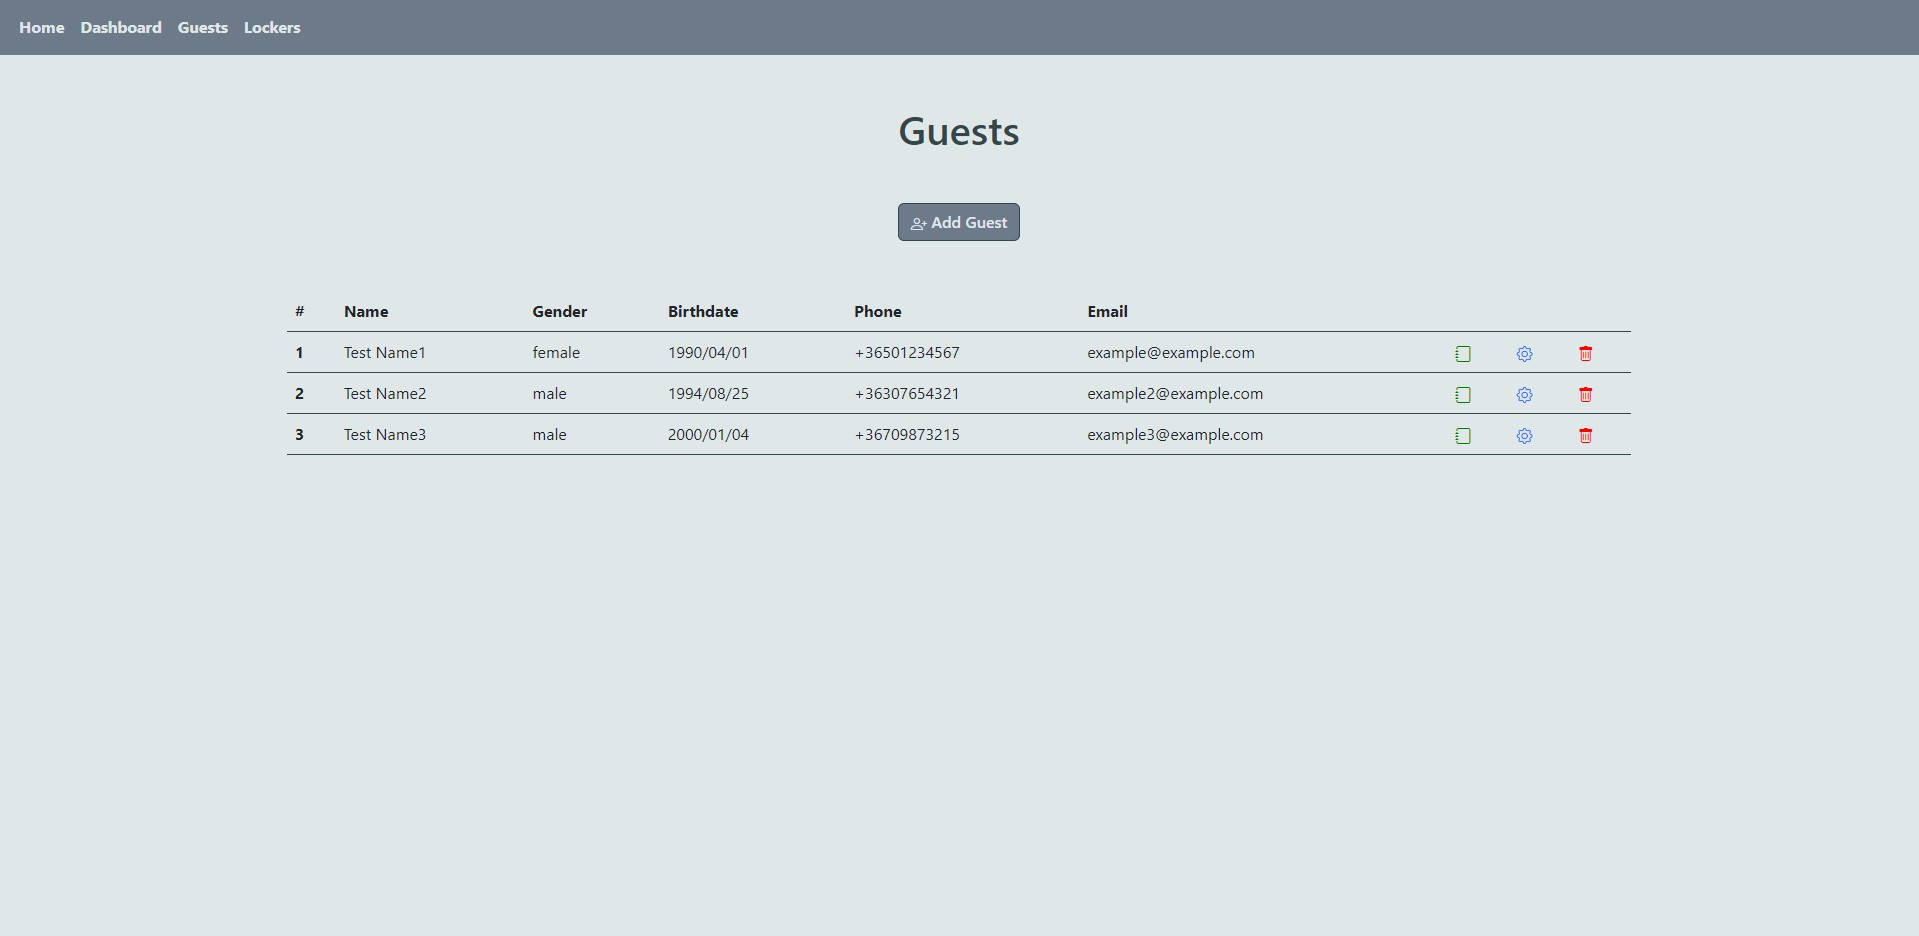
\includegraphics[width=\textwidth]{guests-page}
	\caption{A vendégek kezelőfelülete. }
\end{figure}
\begin{figure}[h!]
	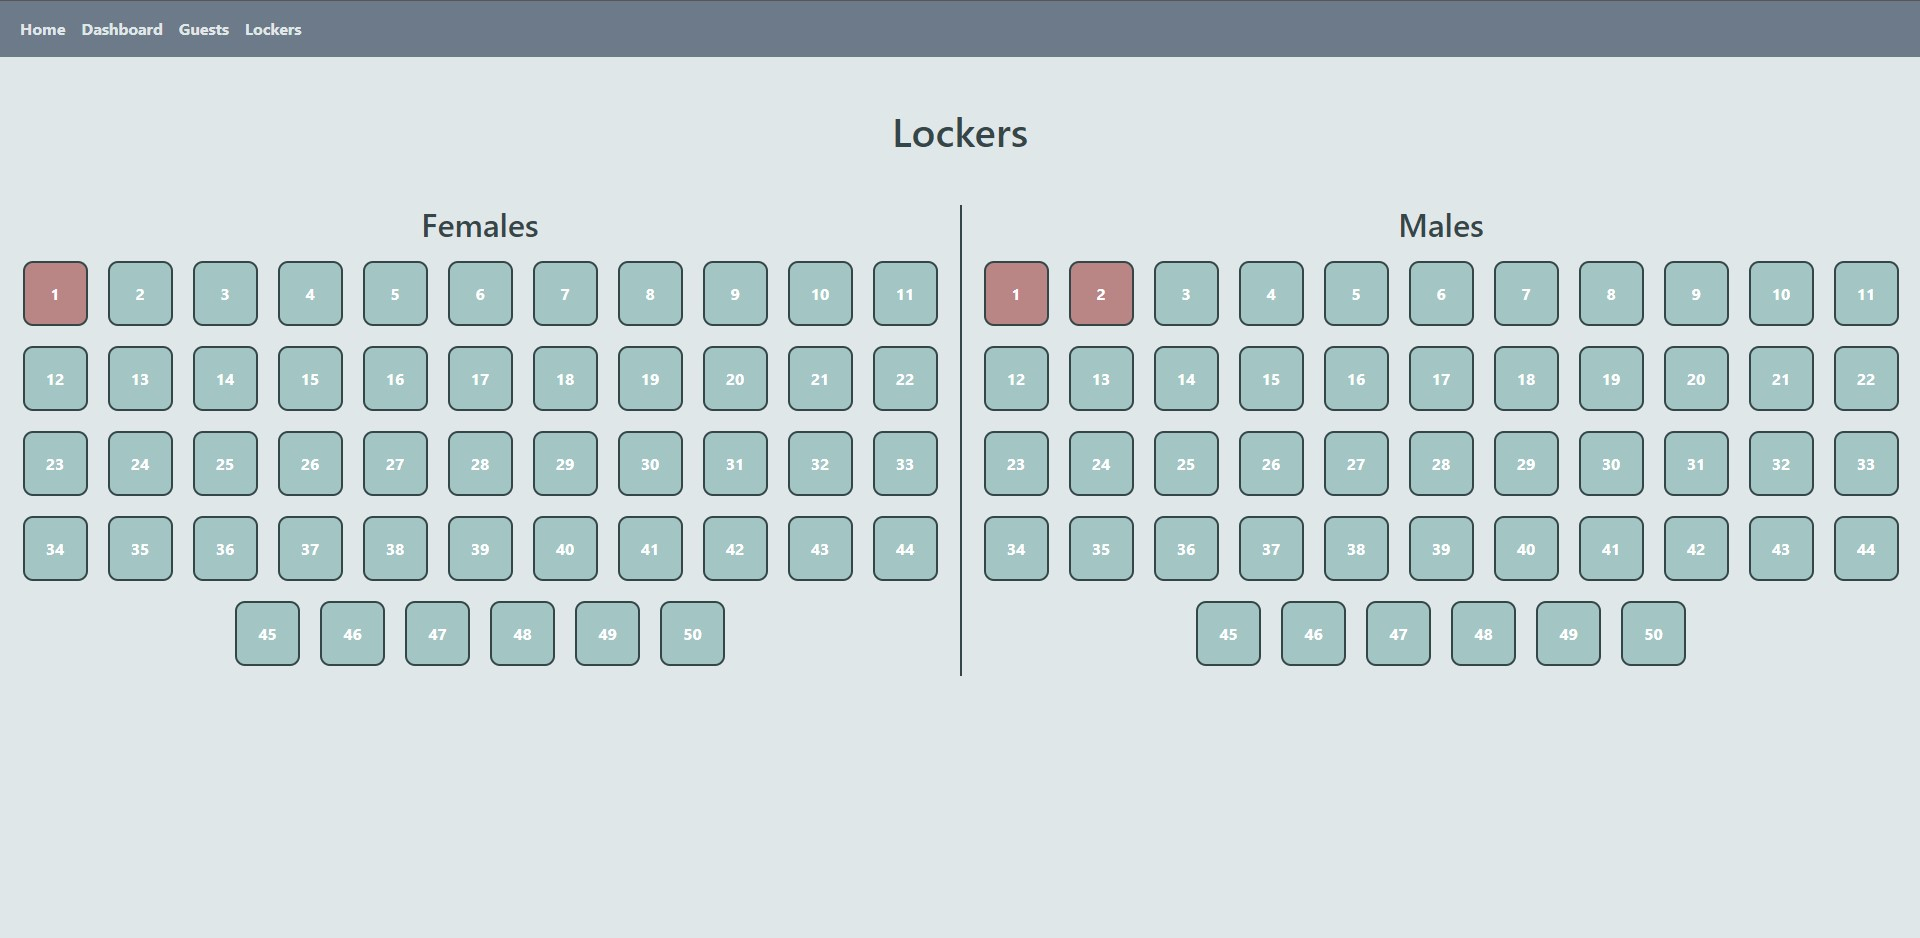
\includegraphics[width=\textwidth]{lockers-page}
	\caption{Az öltözőszekrények státusz oldala. }
\end{figure}

Ezekhez és az említett funkciókhoz tartozó aloldalak mindegyike és a bennük használt komponensek külön \textit{.vue} kiterjesztéssel rendelkező fájlban került implementálásra.
A

\newpage
\section{Az eredmények ismertetése}
\subsection{A fejlesztés tapasztalatai}
\subsection{Mérési eredmények}

\newpage
\section*{Összefoglalás}
\addcontentsline{toc}{section}{Összefoglalás}

%******************példa képek:

%\begin{figure}
%\centering
%\includegraphics[width=0.7\textwidth]{org}
%\caption{Organogram.}
%\end{figure}

%\begin{wrapfigure}{r}{0.4\textwidth}
%\includegraphics[width=0.4\textwidth]{test1}
%\caption{Értékteremtő lánc diagram.}
%\end{wrapfigure}

%\begin{figure}[h]
%\centering
%\begin{subfigure}{0.45\textwidth}
%\includegraphics[width=8cm]{pelda1} 
%\end{subfigure}
%\begin{subfigure}{0.4\textwidth}
%\includegraphics[width=8cm]{pelda2}
%\end{subfigure}
%\caption{A háló $t_1$ tüzelése előtt és után}
%\end{figure}

%******************felsorolas
%\begin{definíció}
%A Petri háló ($PN$) egy ($P, T, E, w, m_0$) rendszer, ahol
%\begin{enumerate}
%\item $P$ a helyek véges halmaza,
%\item $T$ a tranzíciók véges halmaza feltéve, hogy $P \cap T = \emptyset$,
%\item $E \subseteq (P \times T) \cup (T \times P)$ az élek véges halmaza,
%\item $ w: E\rightarrow N^+$ a súlyfüggvény,
%\item $ m: P\rightarrow N$ a token-eloszlás függvény,
%\item $ m_0$ a kezdeti token eloszlás.
%\end{enumerate}
%A Petri háló struktúrát $(P, T, E, w)$ módon jelöljük. (\textit{Peterson., 1981})
%\end{definíció}

%******************felsorolas
%\begin{itemize}
%\item egy adott időszakban egy vevő mennyit vásárolt?
%\item melyik partnernek mennyi ki nem fizetett, vagy lejárt tartozása van?
%\item egy adott termékből mennyi fogyott adott idő alatt?
%\item ki állított ki egy bizonyos számlát?
%\item kik vannak jelenleg bejelentkezve?
%\item kinek van lejárt tartozása és mennyi?
%\end{itemize}

\addcontentsline{toc}{section}{Irodalomjegyzék}

\newpage
\renewcommand{\refname}{Irodalomjegyzék}
\begin{thebibliography}{99}

\bibitem{CS}
C. Scalfani. Functional Programming Made Easier: A Step-by-Step Guide. 2021.

\bibitem{PE}
P. Freeman. PureScript by Example. 2014 - 2017.
\url{https://book.purescript.org/}

\bibitem{VD}
Dr. Vadász Dénes: Programozási paradigmák, programozási nyelvek (letölthető egyetemi oktatási anyag)
\url{https://web.archive.org/web/20150501083657/http://www.iit.uni-miskolc.hu/iitweb/export/sites/default/users/DVadasz/GEIAL401/Progpar-4-fejezet.pdf#}
Hozzáférés dátuma: 2023.04.11.

\bibitem{JM}
John McCarthy: The implementation of LISP. 1996.
http://www-formal.stanford.edu/jmc/history/lisp/node3.html

\bibitem{Sz}
Szuromi Zs.: Programozási paradigmák, kézirat. ME, 1996.

\bibitem{TIO}
The TIOBE Programming Community index. \url{https://www.tiobe.com/tiobe-index/} Hozzáférés dátuma: 2023.04.11.

\bibitem{Java}
A Java nyelv hivatalos honlapja. \url{https://dev.java/learn/lambdas/}  Hozzáférés dátuma: 2023.04.11.

\bibitem{sy}
B. Radojicic.: Imperative to Functional Programming in Java. 2022
\url{https://symphony.is/blog/imperative-to-functional-programming-in-java} Hozzáférés dátuma: 2023.04.11.

\bibitem{JN}
J. Neumann.: Advantages and disadvantages of functional programming. 2022.
\url{https://medium.com/twodigits/advantages-and-disadvantages-of-functional-programming-52a81c8bf446}
Hozzáférés dátuma: 2023.04.12.

\bibitem{PS}
\url{https://www.purescript.org/}

\bibitem{vue}
\url{https://vuejs.org/guide/introduction.html}

\bibitem{py}
J. Sturtz.: Functional Programming in Python: When and How to Use It. Hozzáférés dátuma: 2023.04.20.
\url{https://realpython.com/python-functional-programming/}

\bibitem{cpp}
D. Cravey.: Functional-Style Programming in C++. Hozzáférés dátuma: 2023.04.20.
\url{https://learn.microsoft.com/en-us/archive/msdn-magazine/2012/august/c-functional-style-programming-in-c}

\href{https://learn.microsoft.com/en-us/archive/msdn-magazine/2012/august/c-functional-style-programming-in-c}{D. Cravey.: Functional-Style Programming in C++}.\\ Hozzáférés dátuma: 2023.04.20.

\bibitem{JS_USAGE}
Kliens-oldali programozási nyelvek használatát bemutató statisztika. \url{https://w3techs.com/technologies/details/cp-javascript}  Hozzáférés dátuma: 2023.04.23.

\bibitem{VUE_SUPP}
A Vue.js által támogatott böngészők. \url{https://vuejs.org/about/faq.html#what-browsers-does-vue-support} Hozzáférés dátuma: 2023.04.24.

\bibitem{ES2015_USAGE}
Az ES2015-öt támogató böngészők. \url{https://caniuse.com/es6} Hozzáférés dátuma: 2023.04.24.

\bibitem{VUE_COMPANIES}
Vue.js-t használó nagyvállalatok. \url{https://vuejs.org/about/faq.html#is-vue-reliable} Hozzáférés dátuma: 2023.04.24.

\bibitem{FRAMEWORK_PERF}
Különféle JavaScript alapú keretrendszerek benchmark eredményei. \url{https://rawgit.com/krausest/js-framework-benchmark/master/webdriver-ts-results/table.html} Hozzáférés dátuma: 2023.04.24.

\bibitem{VUE_LW}
A Vue.js könnyed tulajdonságának leírása. \url{https://vuejs.org/about/faq.html#is-vue-lightweight} Hozzáférés dátuma: 2023.04.24.

\bibitem{VUE_SCALE}
A Vue.js skálázhatóságának leírása. \url{https://vuejs.org/about/faq.html#does-vue-scale} Hozzáférés dátuma: 2023.04.24.

\bibitem{VUE_DOCS}
A Vue.js hivatalos dokumentációja, útmutatója. \url{https://vuejs.org/guide/introduction.html} Hozzáférés dátuma: 2023.04.24.

\bibitem{VUE_BOOK}
Olga Filipova: Learning Vue.js 2, 2016.

\bibitem{VITE}
A Vue.js fejlesztéshez használt Vite szerver honlapja. \url{https://vitejs.dev/}

\bibitem{JAVA_ABOUT}
A Java nyelv rövid története. \url{https://www.java.com/en/download/help/whatis_java.html} Hozzáférés dátuma: 2023.04.24.

\bibitem{JAVA_BOOK}
David Flanagan: Java in a Nutshell, 2005

\bibitem{ORACLE_JAVA}
A Java nyelv működése. \url{https://docs.oracle.com/javase/tutorial/getStarted/intro/definition.html}

\bibitem{SPRING_BOOK}
Iuliana Cosmina, Rob Harrop, Chris Schaefe, Clarence Ho: Pro Spring 5: An In-Depth Guide to the Spring Framework and Its Tools, 2017

\bibitem{SPRING_INIT}
A Spring Initializr eszköz. \url{https://start.spring.io/}

\bibitem{pd}
A PureScript nyelv hivatalos dokumentációja.
\url{https://github.com/purescript/documentation} Hozzáférés dátuma: 2023.04.24.

\bibitem{pgit}
A PureScript nyelv hivatalos forráskódja.
\url{https://github.com/purescript/purescript} Hozzáférés dátuma: 2023.04.24.

\bibitem{spago}
A Spago hivatalos dokumentációja.
\url{https://github.com/purescript/spago} Hozzáférés dátuma: 2023.04.24.

\bibitem{purs}
Pursuit. Hivatalos PureScript dokumentáció.
\url{https://pursuit.purescript.org} Hozzáférés dátuma: 2023.04.24.

\bibitem{purs}
\url{https://uizard.io} 

\end{thebibliography}
\end{document}
